\documentclass[12pt]{article}
\usepackage[a4paper, total={15cm,25cm}]{geometry}
\usepackage{titlesec}
\usepackage{graphicx}
\usepackage{float}
\PassOptionsToPackage{hyphens}{url}\usepackage{hyperref}
%\usepackage{fancyhdr}
%\setlength{\headheight}{15pt}
%\pagestyle{empty}
%\fancyhead[L]{110-1 Bio-MEMS Fabrication Homework}
%\fancyhead[R]{鄭泊聲 b07611002}
\usepackage{amsmath}
\usepackage{latexsym}
\usepackage{multirow}
\graphicspath{ {./images/} }
\usepackage[backend=biber, citestyle=numeric, bibstyle=numeric, sorting=none]{biblatex}
\addbibresource{ref.bib}
\usepackage{mathspec}   %加這個就可以設定字體
\usepackage{xeCJK}       %讓中英文字體分開設置
\setCJKmainfont{Noto Serif CJK TC} %設定中文為系統上的字型
\newCJKfontfamily[chineseSans]\CJKsans{Noto Sans CJK TC}
\setmainfont{Sabon}
\setsansfont{IBM Plex Sans}
\setmonofont{Roboto Mono}
\XeTeXlinebreaklocale "zh"             %這兩行一定要加,中文才能自動換行
\XeTeXlinebreakskip = 0pt plus 1pt     %這兩行一定要加,中文才能自動換行
\renewcommand{\baselinestretch}{1.35}
\renewcommand{\figurename}{圖}
\renewcommand{\tablename}{表}
\renewcommand{\abstractname}{摘要}
\renewcommand{\contentsname}{目錄}
\renewcommand{\listtablename}{表格目錄}
%\renewcommand*{\bibfont}{\footnotesize}
\titleformat*{\section}{\Large \bfseries}
\titleformat*{\subsection}{\large \bfseries}
\titleformat*{\subsubsection}{\bfseries}
%\setcounter{tocdepth}{2}

\title{Development of HyperSpectral Imaging system}
\author{鄭泊聲\thanks{College Student Researcher, Center for Condensed Matter Science, National Taiwan University}
\and 指導教授:張玉明\thanks{Distinguished Research Fellow, Center for Condensed Matter Science, National Taiwan University}}

\date{\today}

\begin{document}
    \maketitle
    \section*{致謝}
    特別感謝張玉明老師將本系統的開發交付給我,並在過程中給予無私的支持與指導。
    本系統開發承蒙科技部110學年度大專學生參與專題研究計畫
支持(計畫編號110-2813-C-002-218-M),另感謝實驗室的陳
維良博士、黎文鴻博士帶我了解光學系統的基礎知識,羅詔元博士在LabVIEW程式撰寫給予許多指導,及黃鈺淳在研發過程中鼎力
協助。
    \section*{文件說明}
    本文件的目的在於詳細紀錄系統開發的過程,宗旨是幫助閱讀者了解「為甚麼這裡要這樣設計?」之類的問題。
    若您是本系統的使用者,建議您不需要閱讀此份文件。若您是本系統未來的開發者,且主要的開發領域在於系統的硬體,建議您可以在遇到問題時,到本文件中尋找答案。
    若您是本系統的軟體開發人員,強烈建議您在開始開發前將本文件詳盡閱讀,否則可能會發生許多程式上的誤解,或是發生不知從何偵錯等困境。本文件中所提到的所有程式檔案,皆在主程式專案HIS.lvproj中。

    除此之外,
    \begin{itemize}
        \item 我在軟體發過程中所撰寫的程式,皆有詳盡的說明於此: \href{https://cheng-posheng.gitbook.io/hsi-main-project-api-documentation/}{HSI Main Project API Documentation} \footnote{\url{https://cheng-posheng.gitbook.io/hsi-main-project-api-documentation/}}
        \item .init 檔案的設定方式與參數校正說明,可以在此找到: \href{https://bencer.notion.site/init-file-documentation-for-HSI-system-f05871402b4142f085a79efb22f836e6}{.init file documentation for HSI system} \footnote{\url{https://bencer.notion.site/init-file-documentation-for-HSI-system-f05871402b4142f085a79efb22f836e6}}
    \end{itemize}
    本系統開發的所有程式碼與相關文件,皆可在此Github organization找到: \url{https://github.com/HyperSpectral-Imaging}
    \tableofcontents
    \section{第一階段: 硬體}
    第一階段系統是為了在巨觀尺度下觀測實域影像而設計,在本計畫中也是作為概念驗證與軟體開發的雛型。
    在這個階段中,整個系統主要由以下幾個部建構成:
    \begin{enumerate}
        \item Specim V10E 線光譜儀
                \begin{itemize}
                    \item 搭配 Specim OLE 23(mm) 物鏡
                    \item 光譜範圍: 400-1000 $nm$
                    \item 入射狹縫寬: 30 $\mu m$
                    \item 成像尺寸: Image size: $6.15(spectral) \times 14.2 mm$
                \end{itemize}
        \item Andor iXon DU897 EMCCD
            \begin{itemize}
                \item 512 $\times$ 512 pixels
                \item 8.2 $\times$ 8.2 mm
                \item TE cooler
                \item Electron Multiplying gain
            \end{itemize}  
        \item Suruga Seiki 電動載台
                \begin{itemize}
                    \item 搭配 D120 控制器
                \end{itemize}
    \end{enumerate}
    由於V10E線光譜儀的成像尺寸與iXon的正方形CCD尺寸並不同,因此當兩部儀器接合使用後,有部分的像是我們無法觀測到的,如圖\ref{figure: image size}所示,
    我們將能在系統中能到看到V10E的整個光譜範圍,但觀測物的Y軸方向,卻因為iXon CCD的高度較小,因此無法完整觀測。

    \begin{figure}[t]
        \centering
        \includegraphics[width=0.5\linewidth]{imagesize.jpg}
        \caption{Image size when combined}
        \label{figure: image size}
    \end{figure}

    \begin{figure}[t]
        \centering
        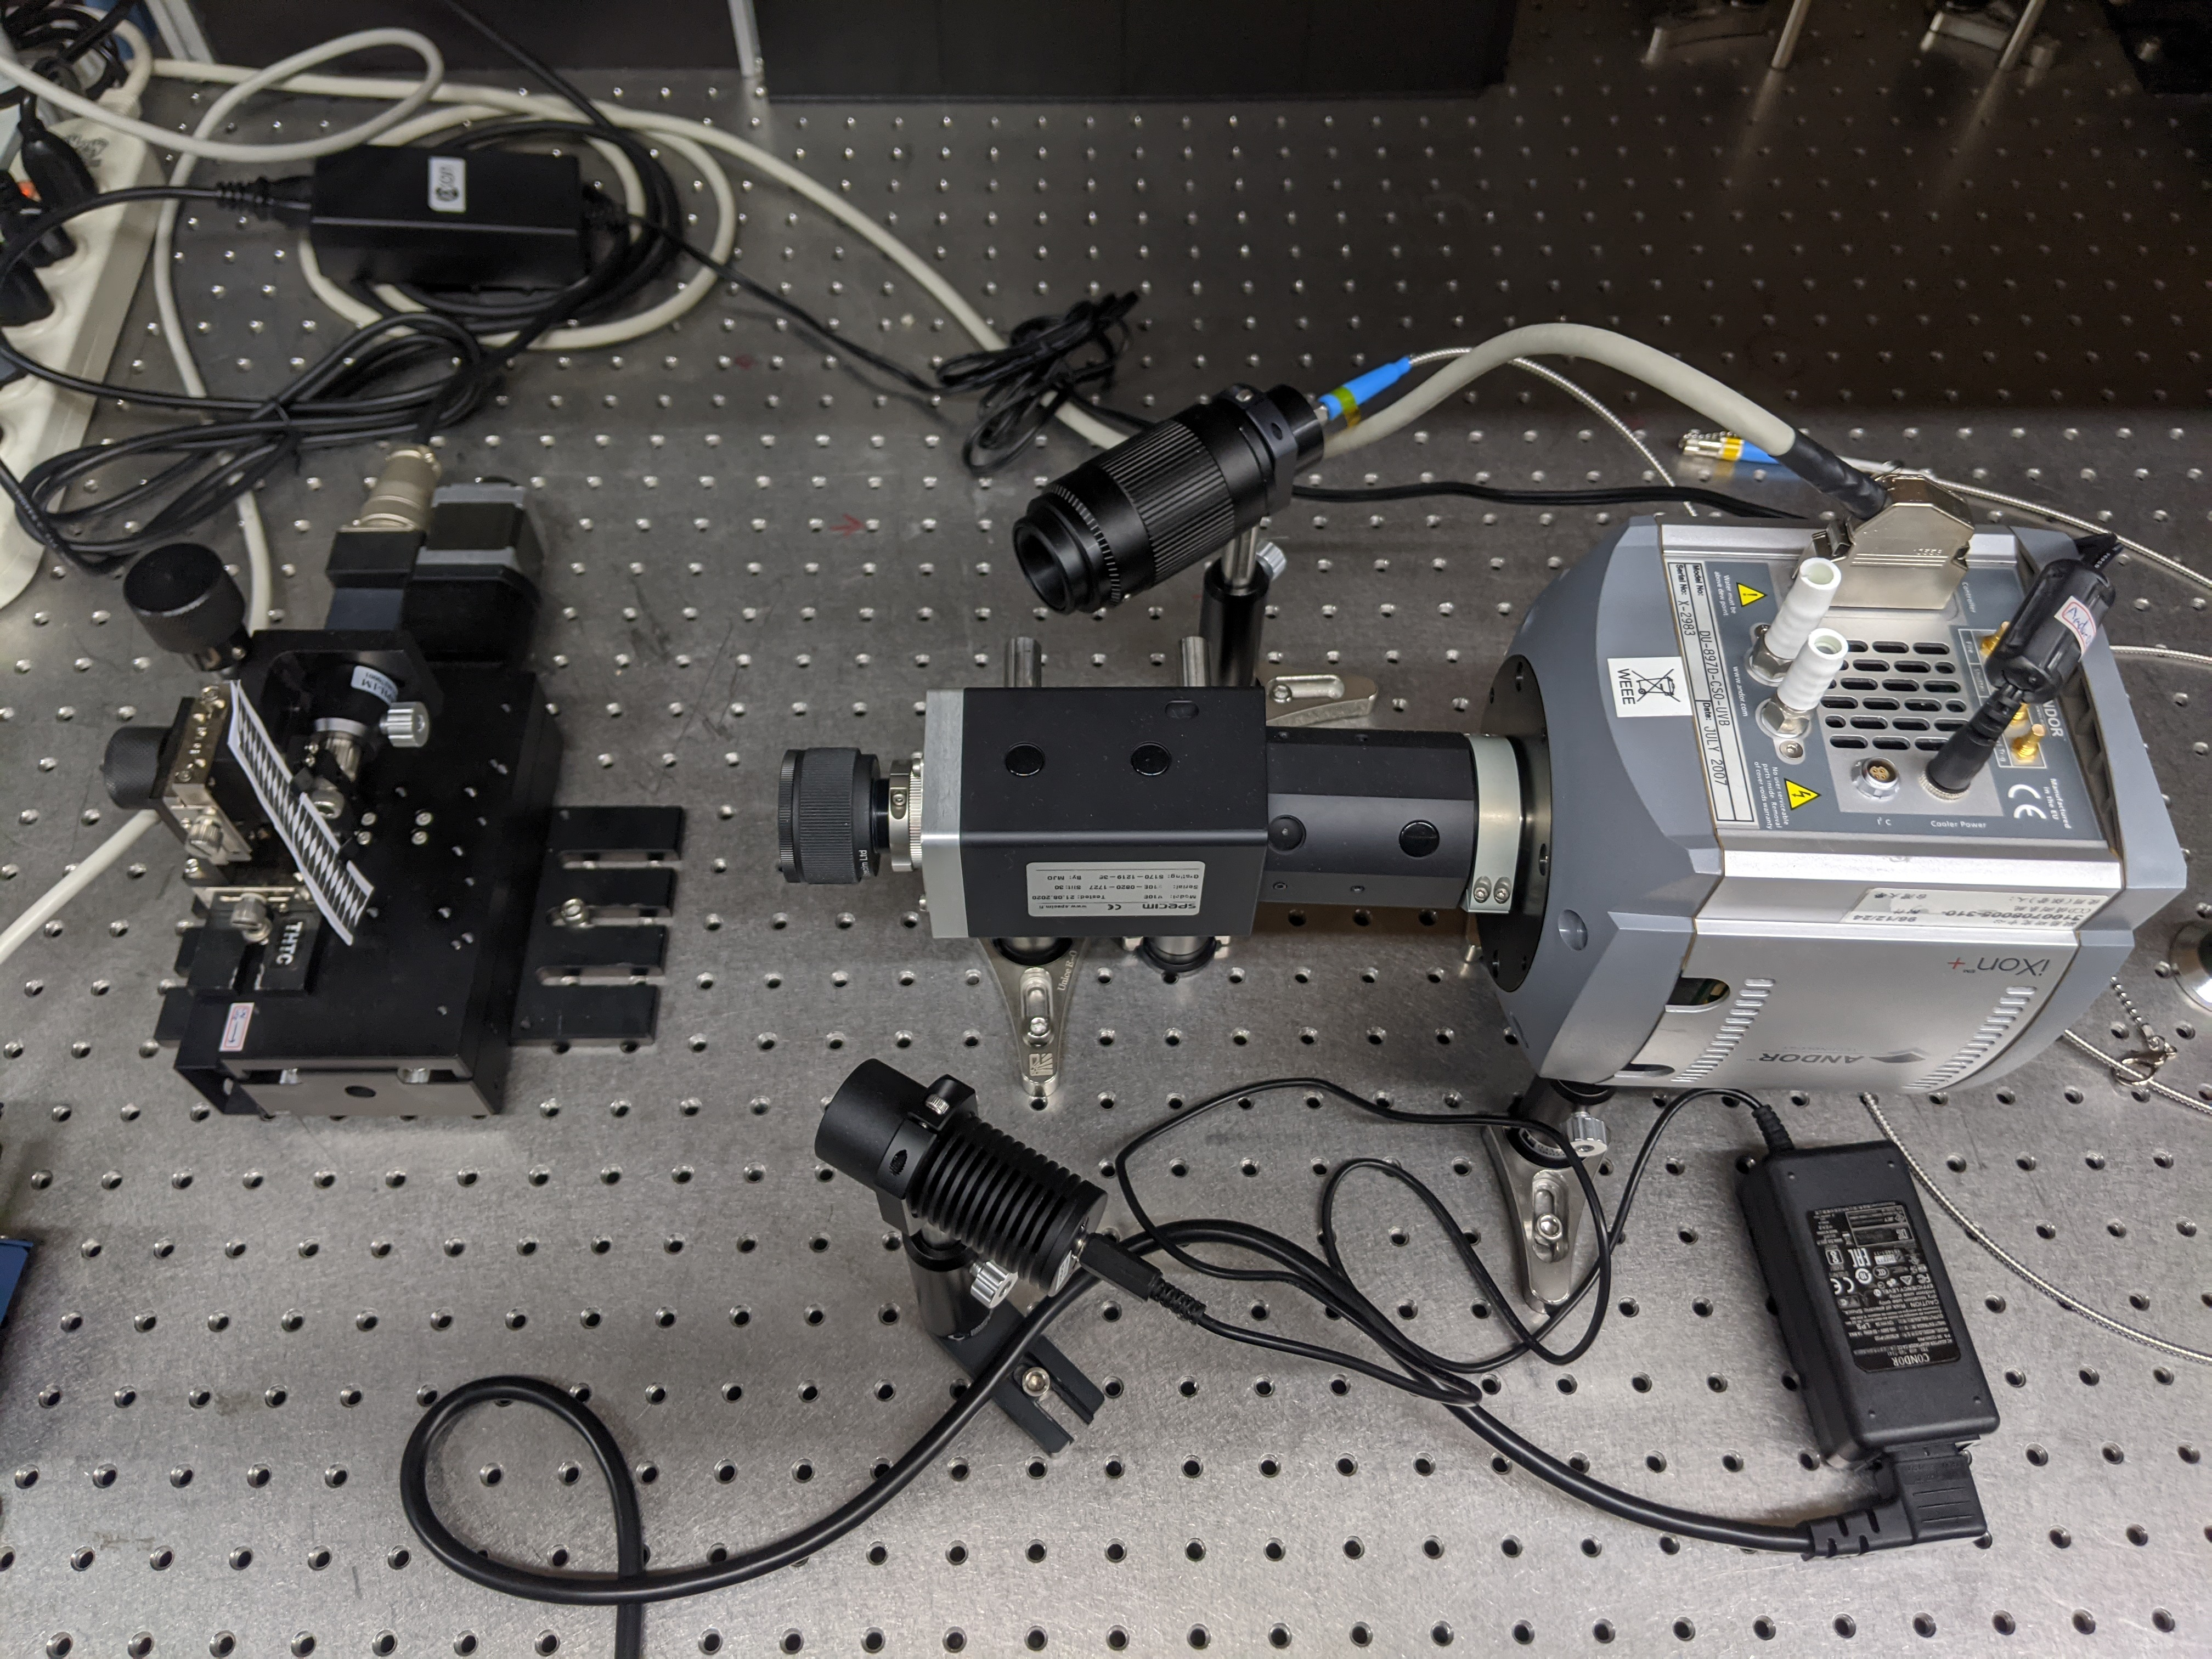
\includegraphics[width=0.65\linewidth]{PXL_20210723_094307842.jpg}
        \caption{Stage, spectrograph, ccd}
        \label{figure: 1 stage setup}
    \end{figure}
    
    圖\ref{figure: 1 stage setup}呈現出第一階段系統的樣貌,在照片中另外可以看到LED光源,從外部的黑色手電筒照射觀測物。

    \subsection{組裝對正與對焦}
    將iXon相機與V10E線光譜儀組裝接合時,有兩件事情必須確認,才能確保所擷取到的影像是正向且準焦的。
    首先,必須確認V10E的像正好在iXon的CCD上匯聚成像。調整方法是,在兩部儀器接合和後,未裝上物鏡的情形下,從線光譜儀的入射狹縫
    ,以一個標準光源打入光線(如我使用Ocean optics Cal-2000 Mercury-Argon 校正用光源),並在電腦上觀測iXon的即時影像。此時由於線光譜儀的入射狹縫完全被標準光源所照亮,
    在影像的畫面上應該看見一條條的直線,每個直線就是光源的一個光譜線。此時即可前後調整V10E後端的鏡組位置(圖\ref{figure: specim bfp lens}),
    直到畫面上的光譜線變得最細、最銳利之時,就代表已經將線光譜儀的像準確成在CCD上了。

    接著,要確保兩部儀器之間的對正,使像跟CCD的方向對齊。只要看畫面上的直線是否完全垂直,就能知道像的方向是否對齊,若直線有傾斜,就要調整V10E與iXon之間的接合角度。以上兩項接合對正都完成後,畫面上的影像應該如圖\ref{figure: align v10e and ixon}所示。

    \begin{figure}[t]
        \centering
        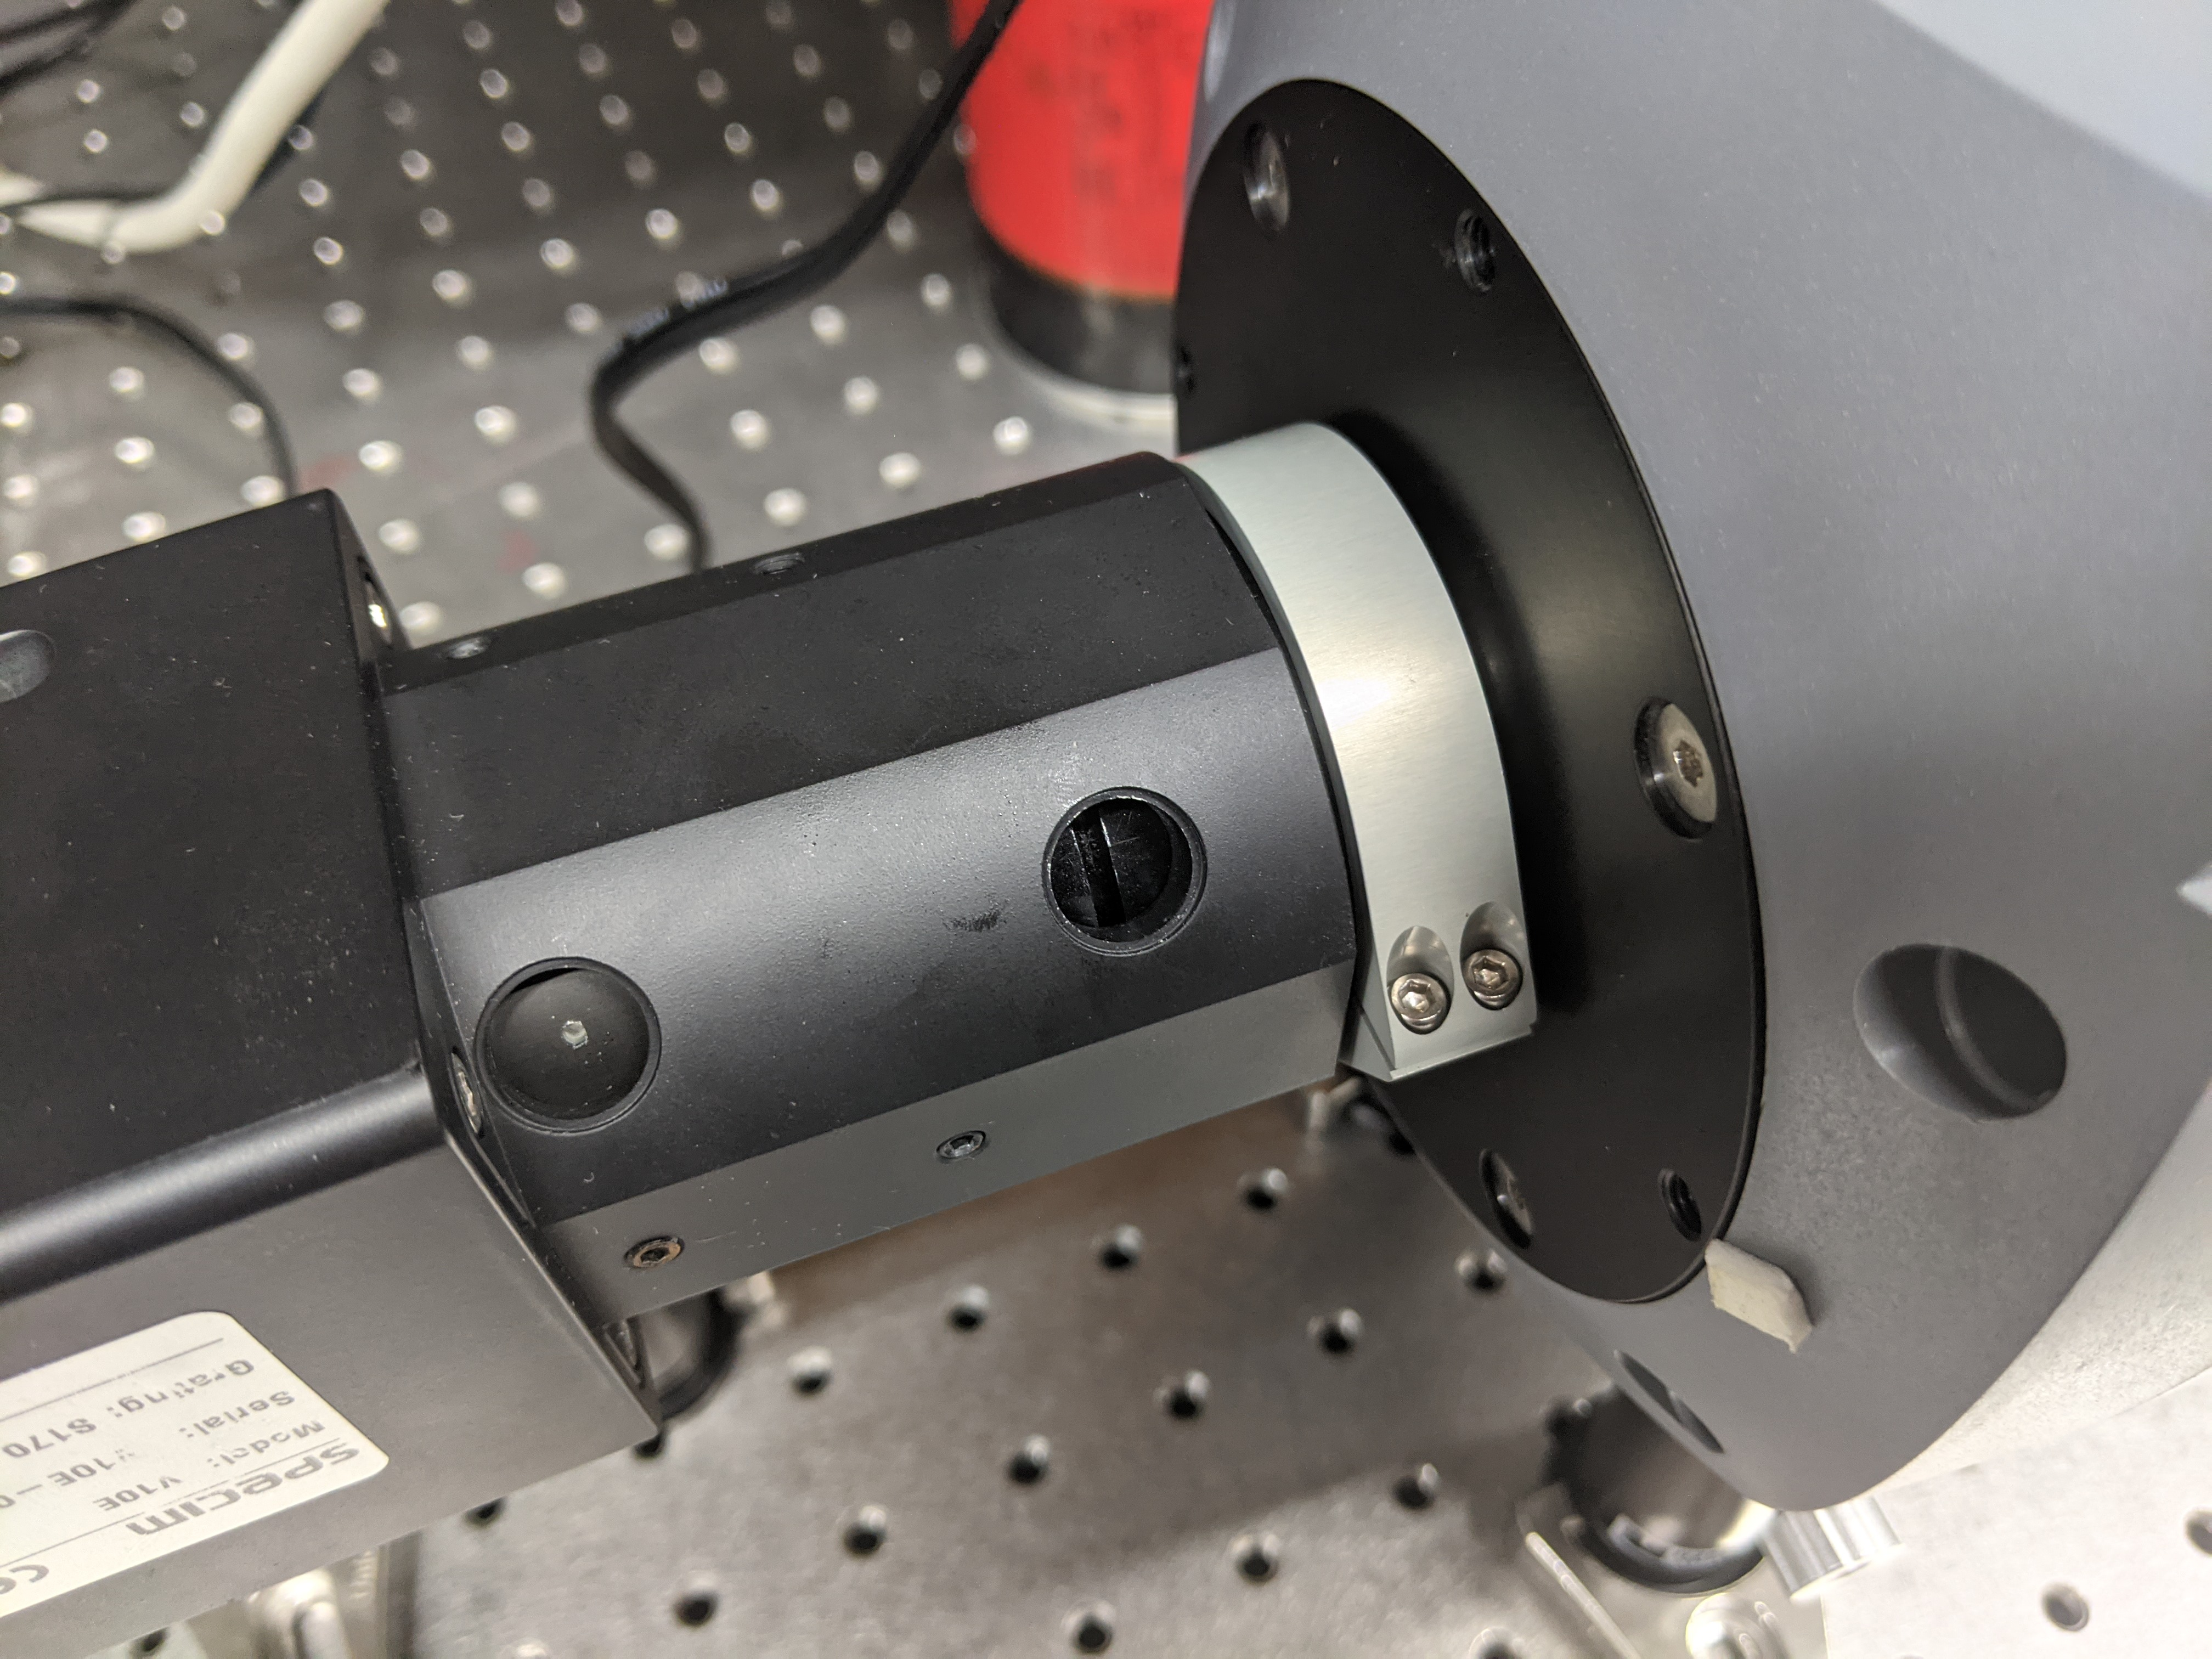
\includegraphics[width=0.65\linewidth]{PXL_20210507_105656554.jpg}
        \caption{Adjust the focusing element of V10E}
        \label{figure: specim bfp lens}
    \end{figure}

    \begin{figure}[t]
        \centering
        
\includegraphics[width=0.8\linewidth]{0423withoutobf.jpg}
        \caption{(on sensor image)Alingment between V10E and iXon}
        \label{figure: align v10e and ixon}
    \end{figure}

    \subsubsection{對焦}
    在巨觀的尺度,可以使用一個Specim 原廠所提供的圖樣(圖\ref{figure: focus pattern})來卻任物鏡的對焦。由於我們無法單純從iXon CCD上的影像判斷目前所觀測的位置,可以先把該圖案放在欲觀測的位置上,
    如圖所示,當線光譜儀觀測該圖案的不同位置時,可以明顯在CCD上看到不同的畫面。(圖\ref{figure: focus})

    觀測物經過物鏡成像後,僅有該像的中間一條細線範圍,能夠進入線光譜儀的入射狹縫,在進入線光譜儀後,該細線上的每一個點,
    會被展開成一光譜,成現在CCD的x軸上。因此,當物鏡準確對焦在這個圖案的正中間時,畫面上所呈現的應該是黑白相間的斑馬紋路,每條紋路的寬度均等,長度與照明光源的光譜有關。而條紋的邊緣應非常銳利,且黑色條紋極細。

    \begin{figure}[t]
        \centering
        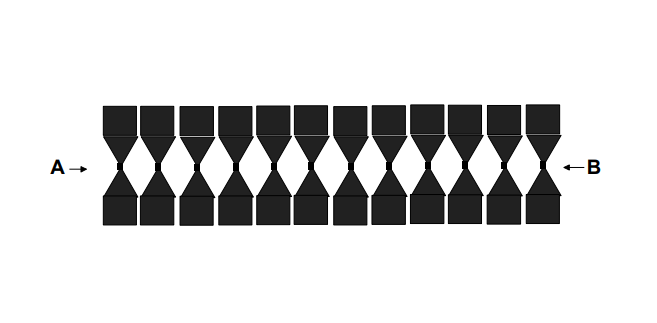
\includegraphics[width=0.8\linewidth]{focusPatern.png}
        \caption{The pattern for checking focus\cite{tn}}
        \label{figure: focus pattern}
    \end{figure}
    \begin{figure}[t]
        \centering
        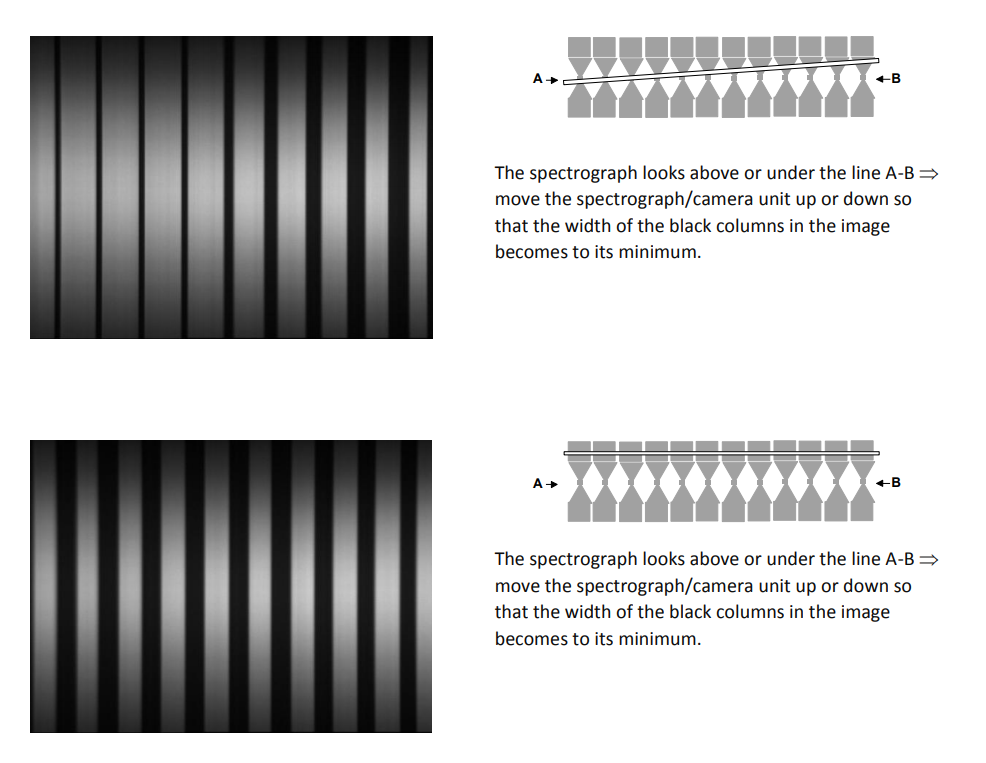
\includegraphics[width=0.6\linewidth]{errorOfFocus.png}
        \caption{(On sensor image)Possible error of focusing. \cite{tn}}
        \label{figure: focus}
    \end{figure}

    \subsection{Order Blocking Filter}
    由於Specim V10E的前玉為一狹縫,光線進入後,理應會發生單狹縫干涉,產生二階影像(Second order image),因此Specim系統中視時尚須搭配一個
    二階濾鏡(Order Blocking Filer),根據原廠的說明書,該濾鏡可以C-Mount安裝,或是直接黏貼在影像感測器上,不論以何種方式安裝,
    皆須盡量靠近影像感測器,實務上與影像感測器不宜超過6mm的距離\cite{manual}。
    \begin{figure}[t]
        \centering
        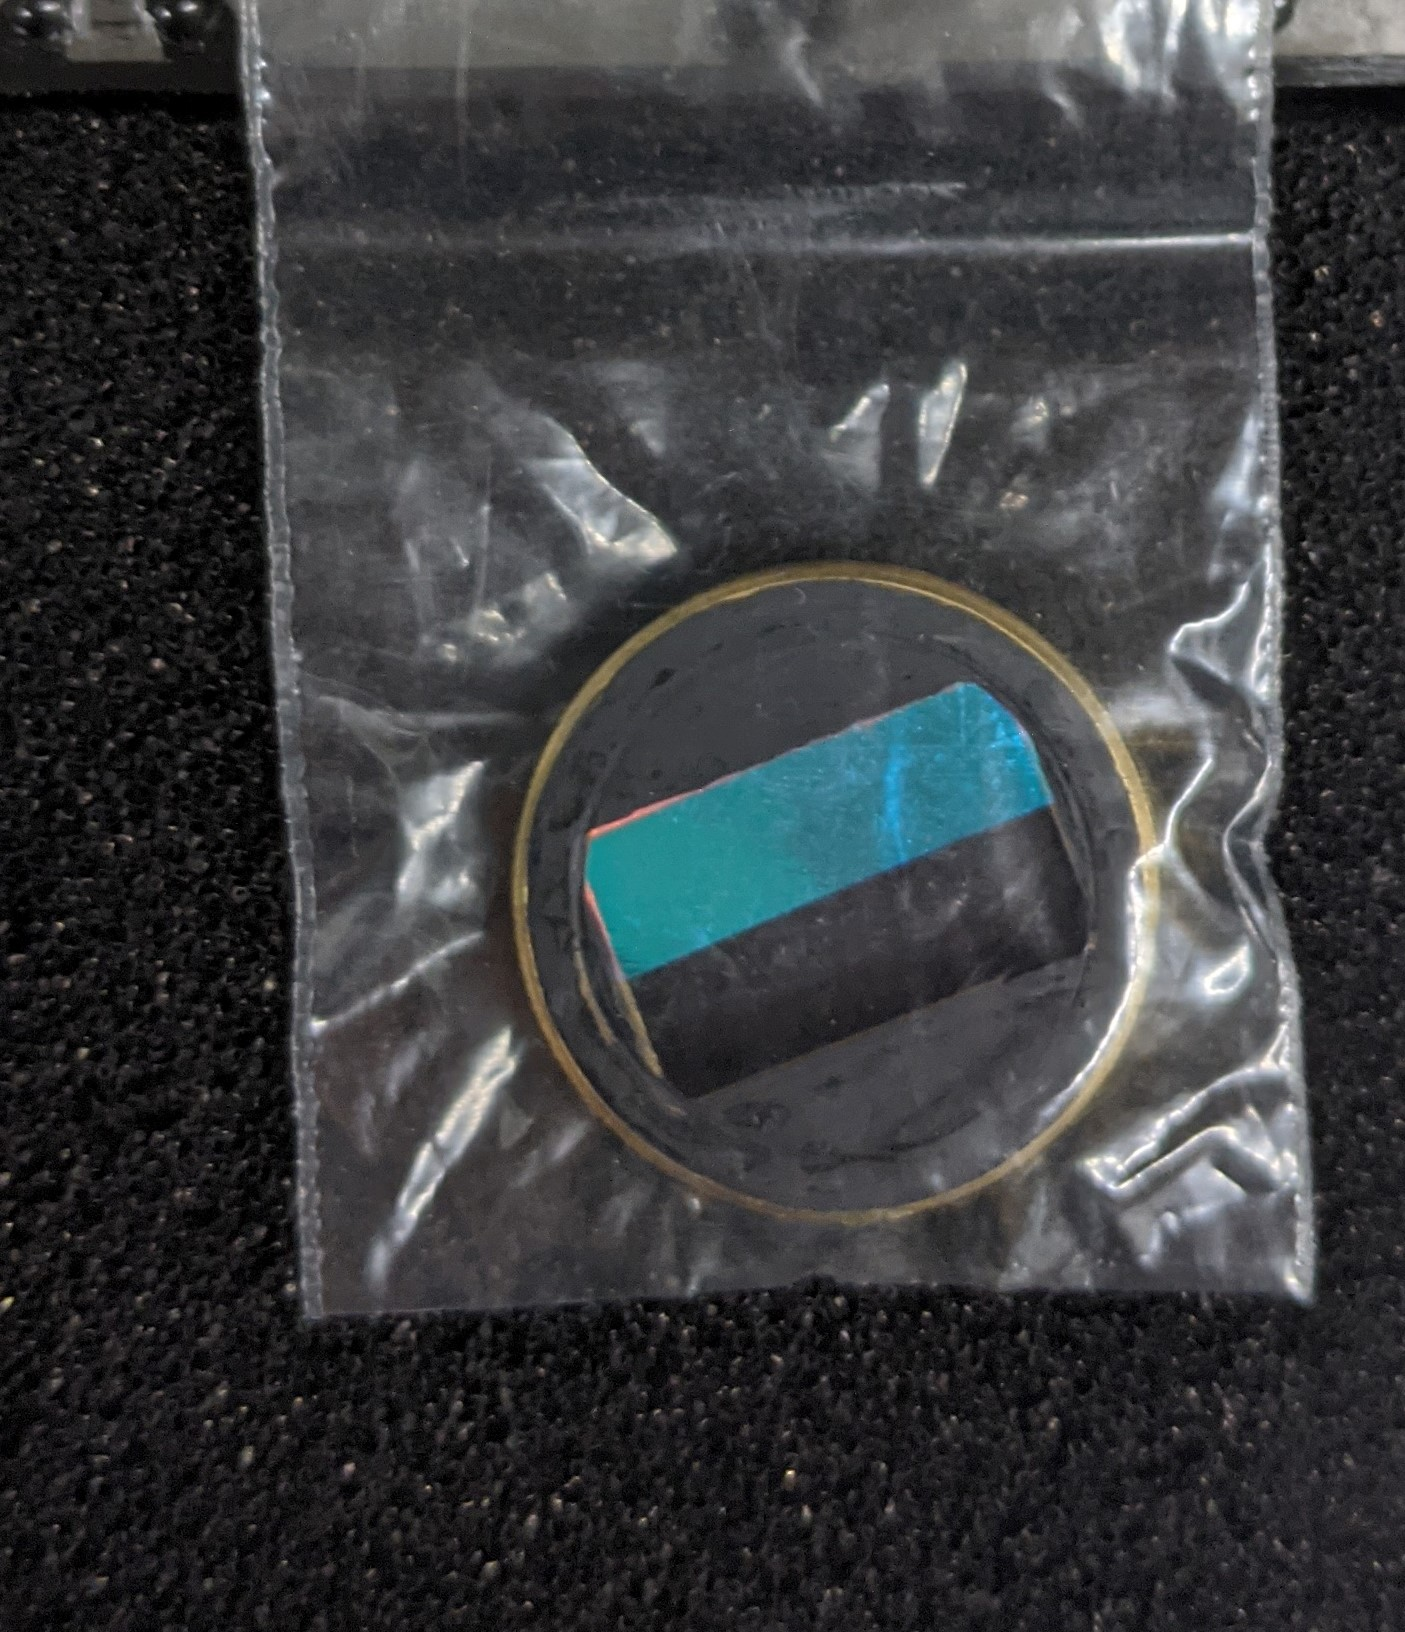
\includegraphics[width=0.5\linewidth]{PXL_20210723_094341395.jpg}
        \caption{The order blocking filter.}
        \label{figure: obf}
    \end{figure}
    觀察該濾鏡的外觀,可發現其阻擋二階干涉影像的方式,應該就是在鏡面上二階影像出現的位置度上塗層進行濾波。由於我們的系統上,不宜將濾鏡直接黏貼在昂貴的iXon EMCCD上,
    原本希望以C-mount方式安裝,但可行的安裝位置與影像感測器的距離都會超過6mm,就算克制專用的c-mount轉接環,仍至少會有約9.55mm左右的距離,我們擔心這樣反而會造成該濾鏡阻擋到原初的一階影像,
    因此最後決定先不安裝該濾鏡,待過後再來檢視二階影像的影響。事實上,在本系統的往後開發過程中,皆沒有在任何影像中看到二階干涉的影響,
    不過這是由於我們未曾使用超過30ms的曝光時間,在更長的曝光時間下,二階干涉是否會造成影響,值得後人加以深究。

    \section{第一階段: 軟體}
    \subsection{三維影像的建立}
    本系統所採用的線掃描 (Line scan or Push-broom) 影像原理,
    可以圖\ref{figure: lineScan}來說明。首先,系統中包含一個簡單的光學顯微鏡,
    能將樣品的像成在一部線光譜儀的入射狹縫上 ( 圖中的 input 
    slit),線光譜儀會同時對狹縫上的每個位置進行光譜量測 ( 圖中
    的 dispersion 示意 ),並在影像感測器上形成一個二維影像 ( 圖
    中 on sensor image),其包含了樣品掃描線上 512 個不同 Y 位
    置的光譜。接著只要再對樣品進行 X 方向的移動掃描,就能將各
    處單線的光譜影像組合成一張完整的高光譜影像 (Hyperspectral 
    image)。

    \begin{figure}[t]
        \centering
        \includegraphics[width=0.75\linewidth]{hsi_from_object_to_cube.jpg}
        \caption{線掃描的原理}
        \label{figure: lineScan}
    \end{figure}

    本系統在拍攝時,實際上從iXon EMCCD上擷取的On sensor image,如圖\ref{figure: linespectrum}所示,其縱軸與分光儀的狹縫同方向,因此也是代表樣品的空間縱軸,
    至於影像的橫軸刻度,則是代表不同波長。換句話說,在這張影像的每一個y位置,都有一條光譜線,在iXon EMCCD 512$\times$512像素的設定下,代表每一張on senson image
    上都有512個不同位置的光譜線。圖\ref{figure: linespectrum}是10x物鏡下,拍攝小型網格圖樣的影像,因此可以看見途中的亮帶與暗帶交錯。

    \begin{figure}[t]
        \centering
        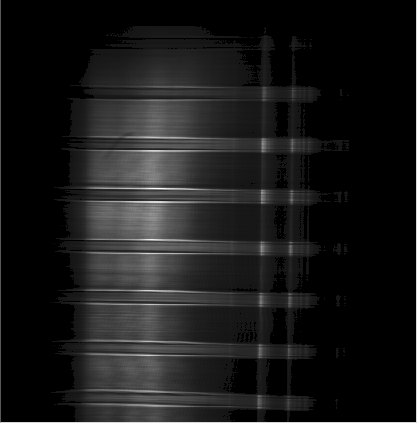
\includegraphics[width=0.5\linewidth]{lineSpectrum1213LDLS.png}
        \caption{網格的線掃描影像}
        \label{figure: linespectrum}
    \end{figure}

    實際上進行掃描時,只要在樣品上不同位置的掃描線擷取影像,就能得知樣品上每個位置的光譜資訊。每張線掃描影像皆是512$\times$512像素的二維影像,
    在掃描後,會得到數張這樣的二維影像,疊合後成為一張三維的影像,在程式中,是以三維的矩陣形式處裡。一開始所疊合而成的三維影像,其x,y,z軸分別為波長、樣品y、樣品x軸,
    與實際的樣品空間座標有出入,因此必須將矩陣的x與z軸調換(transpose),才能產生出一個與樣品空間相同的影像。該影像即是由512張(由於on sensor image在波長方向有512個pixel)各個波長下的樣品二維影像所組成。

    \subsection{影像儲存}\label{section: saveTiff}
    掃描完成後的三維矩陣,我們將其儲存為TIFF影像格式。TIFF全名維Tagged Image File Format,顧名思義,其檔案中能儲存影像與描述影像的各式標籤(Tag)。
    除此之外,Tiff格式支援儲存多個的影像在一個檔案中,故我們能將三維矩陣的每一層二維影像,都儲存在同一個檔案中。

    Tiff檔案大致可分為兩部分,前半部分儲存的是檔案中每一張影像的標籤,描述了各式的影像資料,包括公版的影像資料標籤,如影像的像素數與位元等,也包括了我們自行加入的其他影像資料標籤,
    如每一層二維影像所在的波長,即是以一個一維陣列的方式儲存維一個自定義的影像資料標籤。

    檔案的後半部分,才是各張影像的實際資料。在我們的系統中,每個檔案一慮都會包含512張不同波長下的影像,這些影像也各都會有自己的一組影像資料標籤,這512組影像資料標籤也是都儲存在前半部分。

    我們使用實驗室過去留下的公版tiff labview library來進行影像檔案的儲存與其中影像資料標籤的管理,在開發初期遇到該library內資料寫入檔案時,端序(byte order)不一致的問題,有些資料是以大端序(big endian),
    寫入,有些是以小端序(little endian)寫入,為了配合實驗室Analyser軟體,我們最後一慮皆使用小段序寫入資料。另外,將data cobe寫入檔案時,若將三維矩陣直接寫入,會有array index倒置的問題,正確的寫入方式應該是以for迴圈依序將data cube內的單張影像一張一張寫入。

    \subsection{座標校正}
    \subsubsection{空間x軸校正}
    空間x軸的校正,旨在得知影像上x方向對應到的實際尺寸,與每一個像素在實際空間所在的位置。由於本系統是沿著x方向進行掃描,在電動載台移動到指定位置後,才擷取一張線掃描影像,由於電動載台的位置是已知的,因此也能夠知道自然每個x方向像素所在的實際位置。
    不過在設定電動載台移動距離時,還須注意到掃描線在樣品上實際的寬度,雖然很微小,但仍是存在。依據Specim的說明書,樣品上掃描線的實際寬度,可以
    \begin{equation*}
        W=\frac{W_s\times D}{f}
    \end{equation*}
    來計算,其中$W_s$是狹縫的寬度,$D$是樣品與鏡頭的距離,$f$則是物鏡的焦距。如果電動載台掃描時移動的距離比該寬度還小,實際上就代表每條掃描線之間有重疊,因此在軟體設計上會提示使用者依據此式算是計算出的建議掃描步進。
    $W_s$、$D$、$f$則分別以知名儲存在ini檔案中,以協助軟體計算。
    \subsubsection{空間y軸校正}
    與尚述相同,空間y軸的校正,旨在得知影像上y方向對應到的實際尺寸,與每一個y軸像素於實際空間中所在的位置。實務上要校正y軸,就是要得知入射狹縫上的像在樣品上的實際尺寸。由於狹縫上的像已可視為是一維的影像,所以也可說是要得知狹縫高實際上在樣品上所應的長度。
    在本階段的巨觀尺度下,可以拍攝已知高度與刻度的圖樣,如下圖\ref{figure: self pattern},的on sensor image,並在其上計算y方向亮暗帶交錯的次數,即可得知狹縫的y視野,在後面微觀的系統下,
    我們以已知方格大小的銅網螢光片來計算,也可得知影像y軸的實際尺寸,並將其儲存在ini檔的項目中。
    \begin{figure}[t]
        \centering
        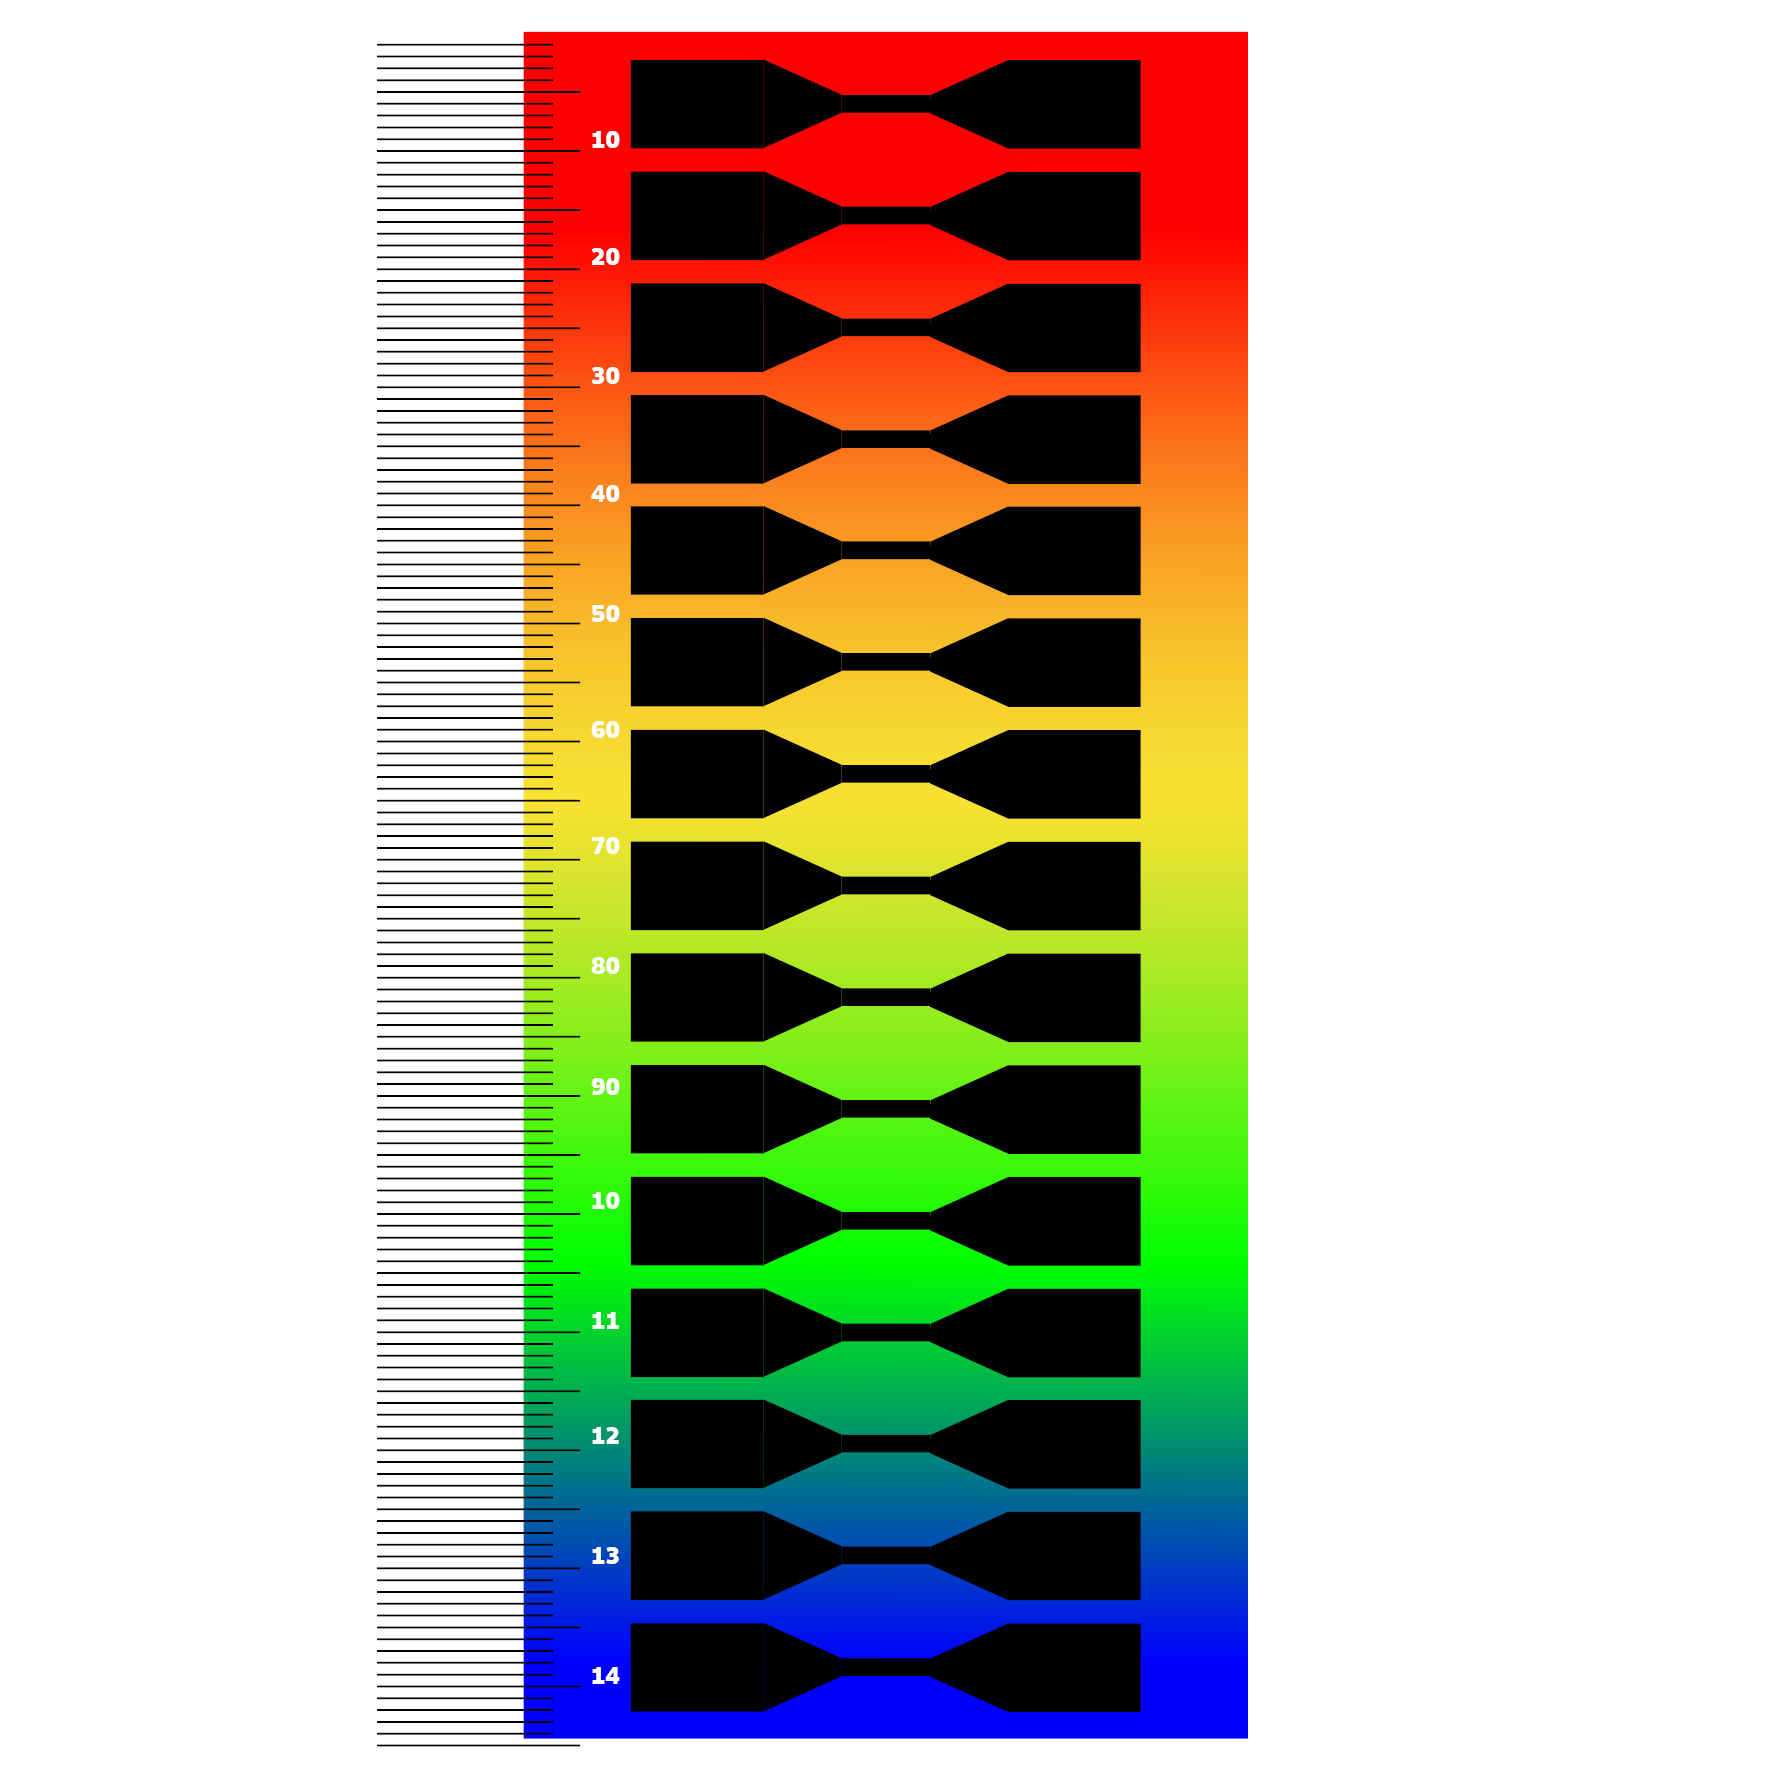
\includegraphics[width=0.4\linewidth]{patternColor.jpg}
        \caption{A self-designed pattern for focusing and calibration.}
        \label{figure: self pattern}
    \end{figure}
    \subsubsection{波長軸(z)校正} \label{section: z cali}
    所謂波長軸的校正,就是要知道on sensor image上每個x軸像素所代表的波長,或說是最終三維影像資料中,每一層二維影像所在的波長。在本階段巨觀系統硬體下,校正方式是將
    標準光源(cal-2000)自物鏡前方直接打入,並在iXon隨附的Solis軟體中得出on snesor image在x方向的平均line profile,
    接著精確讀出每個波峰所在的x像素,並與標準光源的已知光譜以線性回歸推出進行減量線,其斜率與截距儲存在ini檔的項目中,軟體即會自動計算並調整螢幕上所顯示的波長。
    關於Solis軟體的操作細節,請參閱原廠的說明書,在此以Cal-2000為校正光源,說明如何透過Solis軟體擷取校正光譜軸所需的步驟。
    \begin{enumerate}
        \item 當iXon的感測晶片被Cal-2000照滿時,應該觀測到如圖\ref{figure: fitting_image}的影像。
        \item 此時以軟體右上方的控制按鈕,將顯示模式調整為2D,或是以圖\ref{figure: fitting_rowplot}的右鍵選單,在任選位置上畫出Row Plot,即可得到如圖\ref{figure: fitting_profile}的畫面。該畫面是原影像的Horizontal line profile,
        由於影像的橫軸是光譜軸,因此其也就是Cal-2000的光譜在iXon上的分布。
        \item 用滑鼠點選光譜,可以看到十字形符號出現在光譜上。用鍵盤的左右鍵,即可移動十字形符號的位置。內視窗的下方會顯示目前十字形位置所在的X方向像素編號,如圖\ref{figure: fitting_profile}中的$X:$。
        \item 透過鍵盤左右鍵,找出數個波鋒的X方向像素編號,並比對Cal-2000的光譜圖,即可知道這幾個像素編號所代表的波長。以波長對像素編號作圖,即可得出圖\ref{figure: fitting}。
    \end{enumerate}
    \begin{figure}[ht]
        \centering
        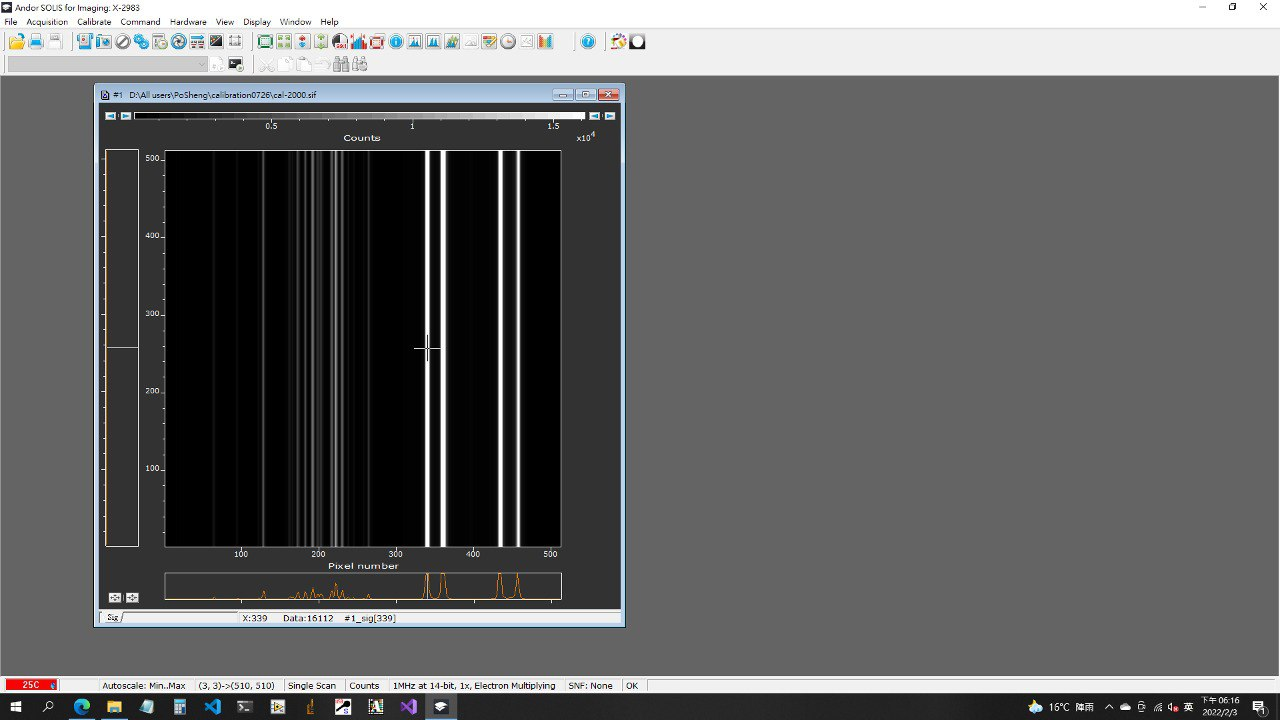
\includegraphics[width=\linewidth]{cal2000examImage.jpeg}
        \caption{以cal-2000進行校正}
        \label{figure: fitting_image}
    \end{figure}
    \begin{figure}[ht]
        \centering
        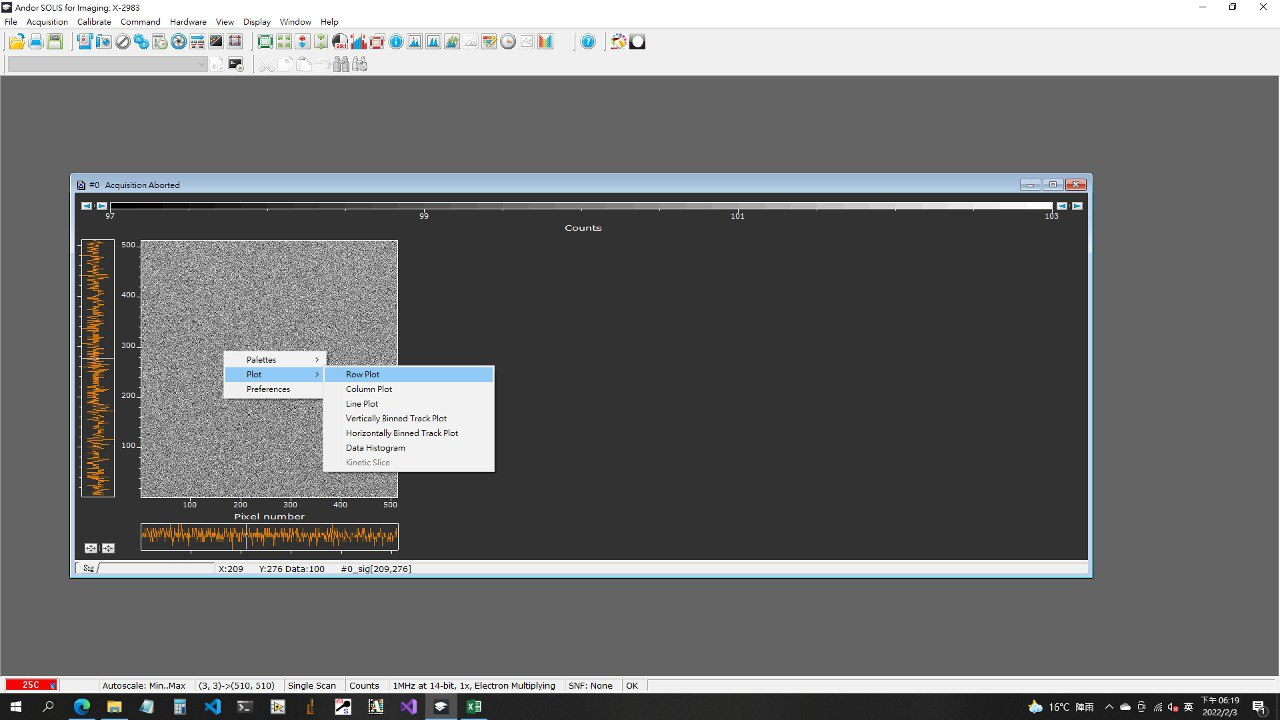
\includegraphics[width=\linewidth]{rowPlot.jpeg}
        \caption{以cal-2000進行校正}
        \label{figure: fitting_rowplot}
    \end{figure}
    \begin{figure}[ht]
        \centering
        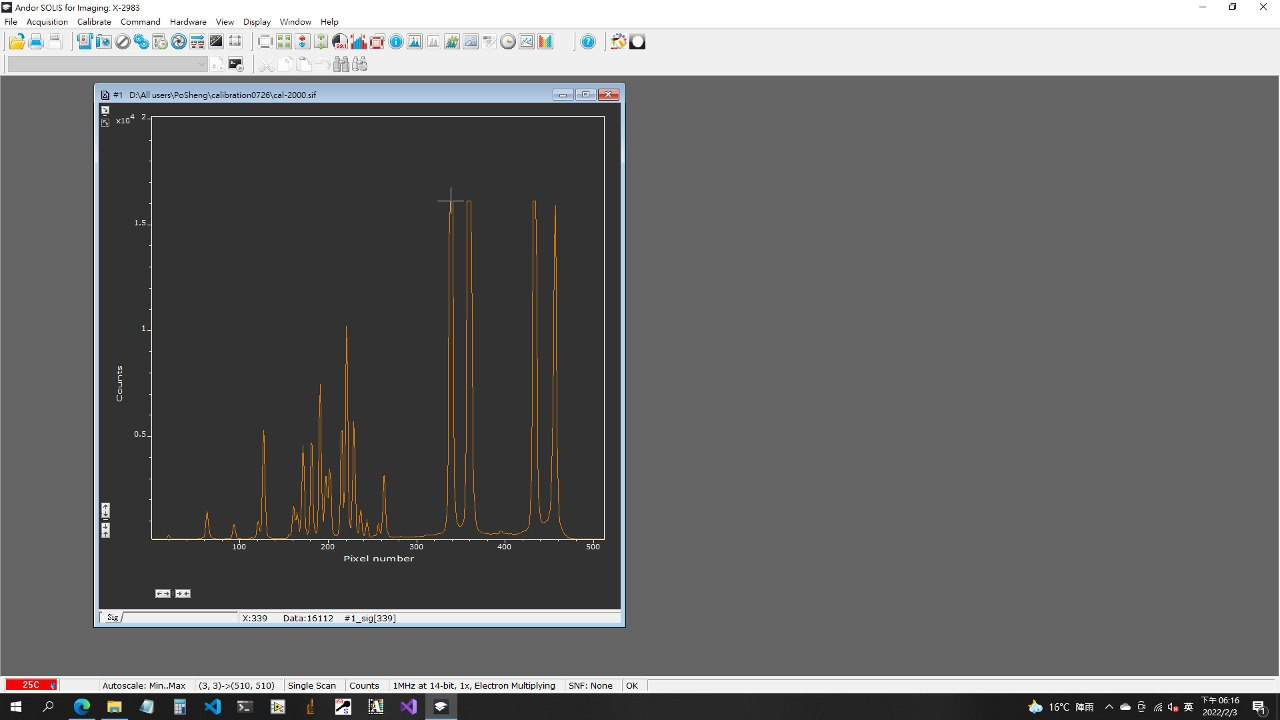
\includegraphics[width=\linewidth]{HLineProfile.jpeg}
        \caption{以cal-2000進行校正}
        \label{figure: fitting_profile}
    \end{figure}
    在接下來微觀系統的校正,方法亦相同,但由於微觀系統採用內部照明的方式,標準光源以光纖方式進入系統,此時僅需在樣品處放置一個銀鏡,即可量測標準光源離開物鏡打到銀鏡後的反射光譜。
    
    \begin{figure}[t]
        \centering
        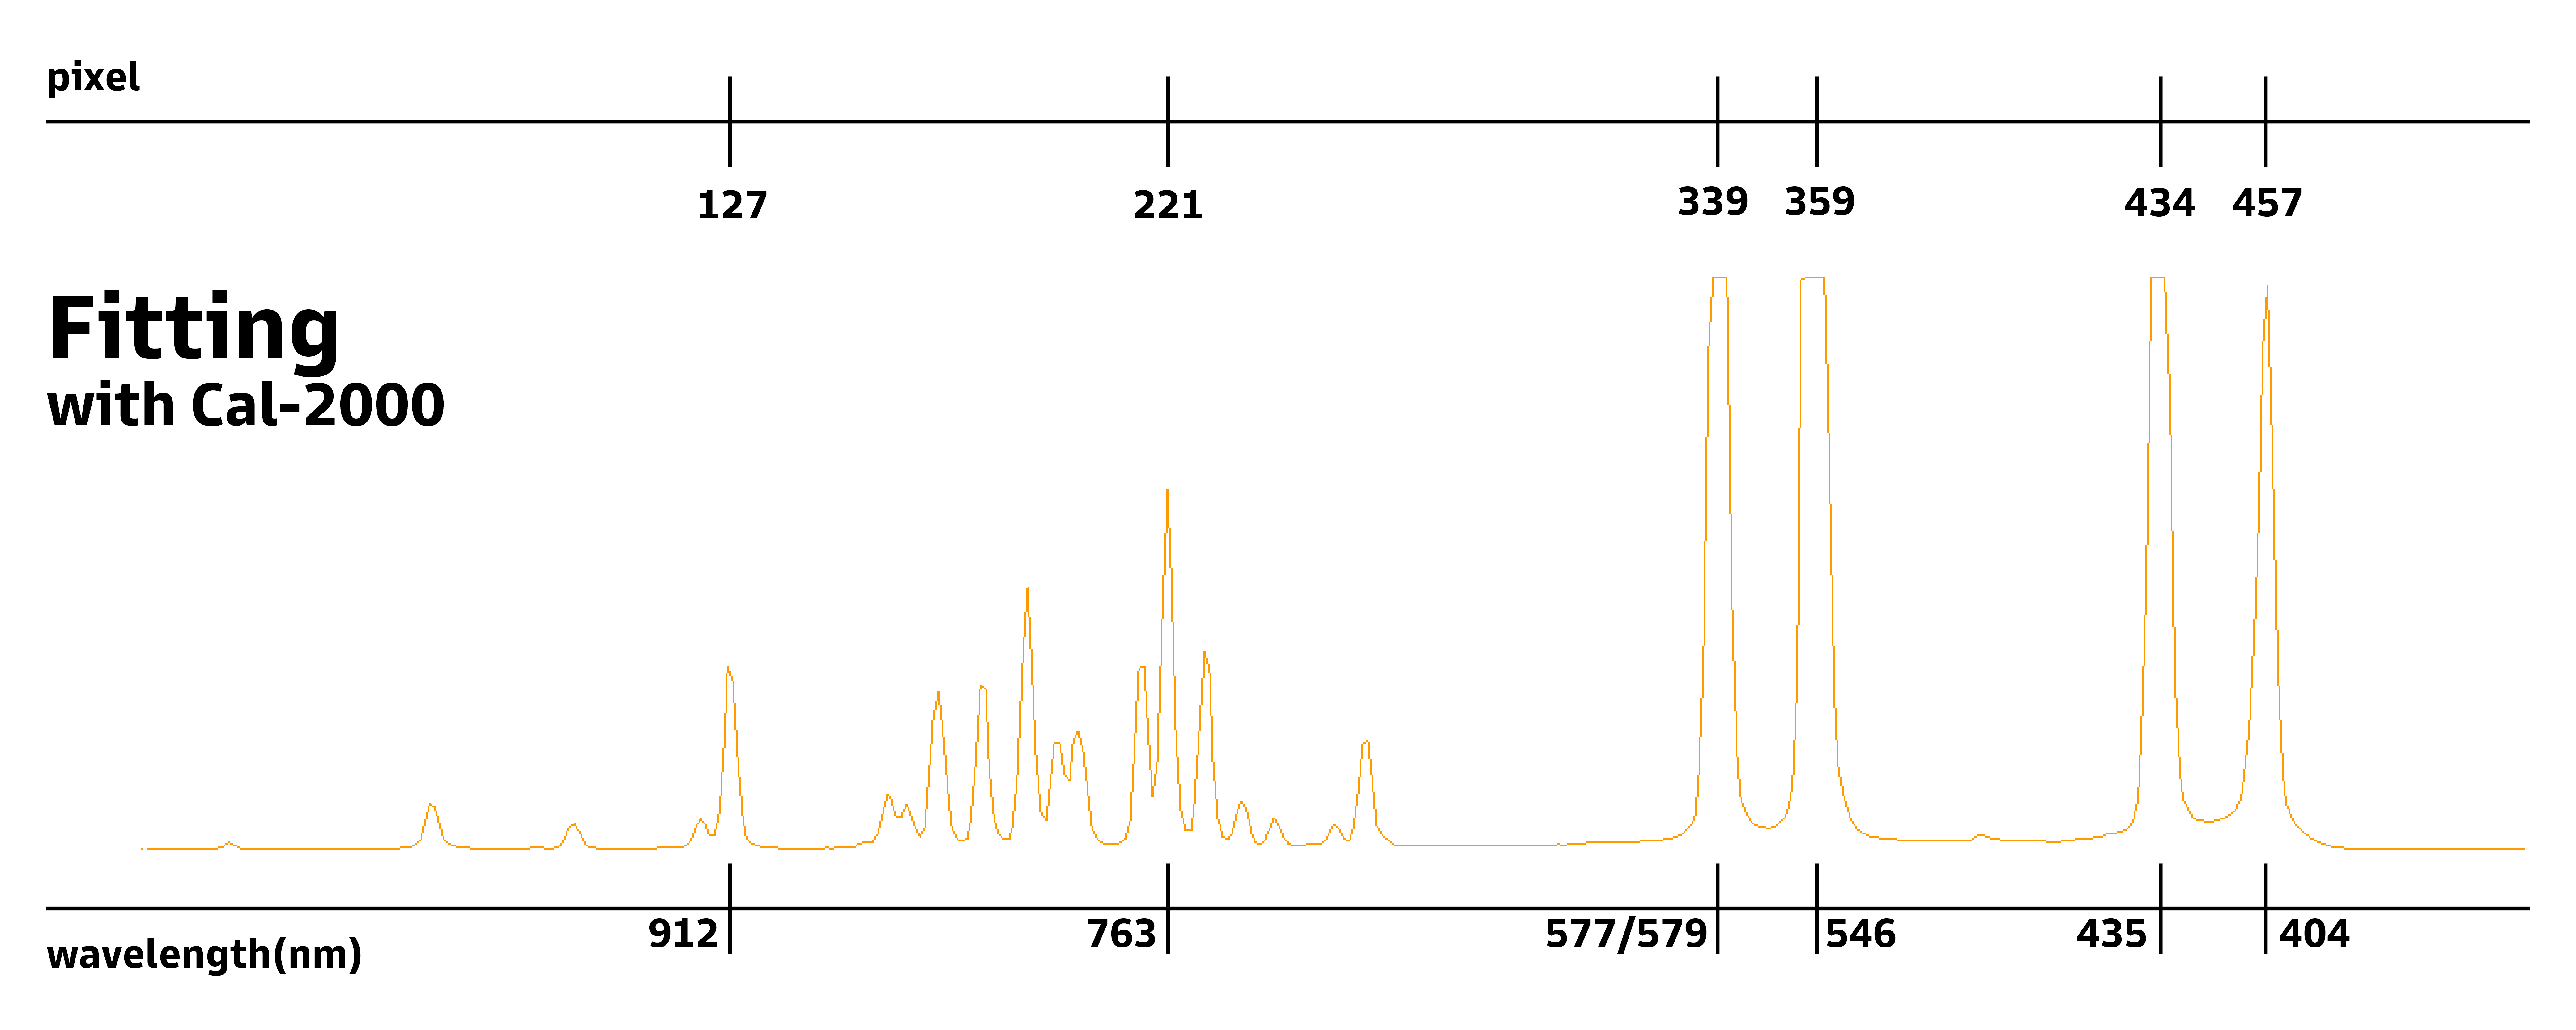
\includegraphics[width=\linewidth]{fitting.jpg}
        \caption{以cal-2000進行校正}
        \label{figure: fitting}
    \end{figure}
    \begin{figure}[t]
        \centering
        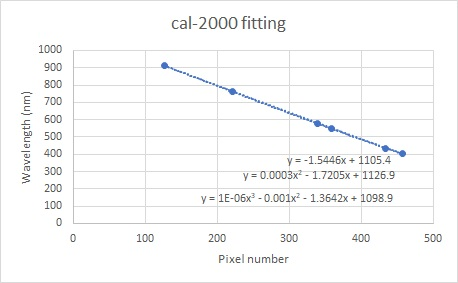
\includegraphics[width=\linewidth]{cal-2000fitting.jpg}
        \caption[]{波長軸校正減量線\protect\footnotemark}
        \label{figure: fit curve}
    \end{figure}
    \footnotetext{請注意,校正時必須導出與本圖相似的負斜率減量線,若導出的減量線為正斜率,可以在Solis軟體中Acquisition setting設定flip image。}
    \section{第二階段: 硬體}
    第二階段的系統,主要目的在於將同樣的線掃描技術,應用於微觀尺度,硬體上的變更,首要就是將原本第一階段所採用的23mm camera lens,置換成一具簡單的光學顯微鏡。我們採用了Olympus 的10x顯微物鏡,
    並搭配15 cm的tube lens,將放大過後的樣品影像成在分光儀的入射狹縫上,至於分光儀與iXon影像感測器的設置,則沒有不同。

    除此之外,系統的照明方式也有改變。原初以外部照光的方式,對於所需照明範圍相對較小的顯微影像來說,會浪費較多光源,也不適合進行雷射螢光等觀測,
    因此將照明方式改為內部照明,系統上有兩個光纖collimator,能夠彼此切換。光源經過tube lens匯聚在物鏡的背焦面上,通過物鏡後變成平行光,以期照射在樣品上的光線最為均勻。

    裝設物鏡的鏡架,能夠上下移動以進行對焦,光源的tube lens也能微調位置。物鏡的tube lens雖然裝設在可調的鏡筒內,但不應任意移動。至於電動載臺的裝設與使用,則沒有不同。
    系統上另外再成像進入分光儀狹縫前,已一片半反射鏡將OM影像投至一臺Canon M200相機中,借助其APS-C尺寸的感光元件,能夠完整顯示出OM的視野,以幫助使用者尋找ROI。
    \begin{figure}
        \centering
        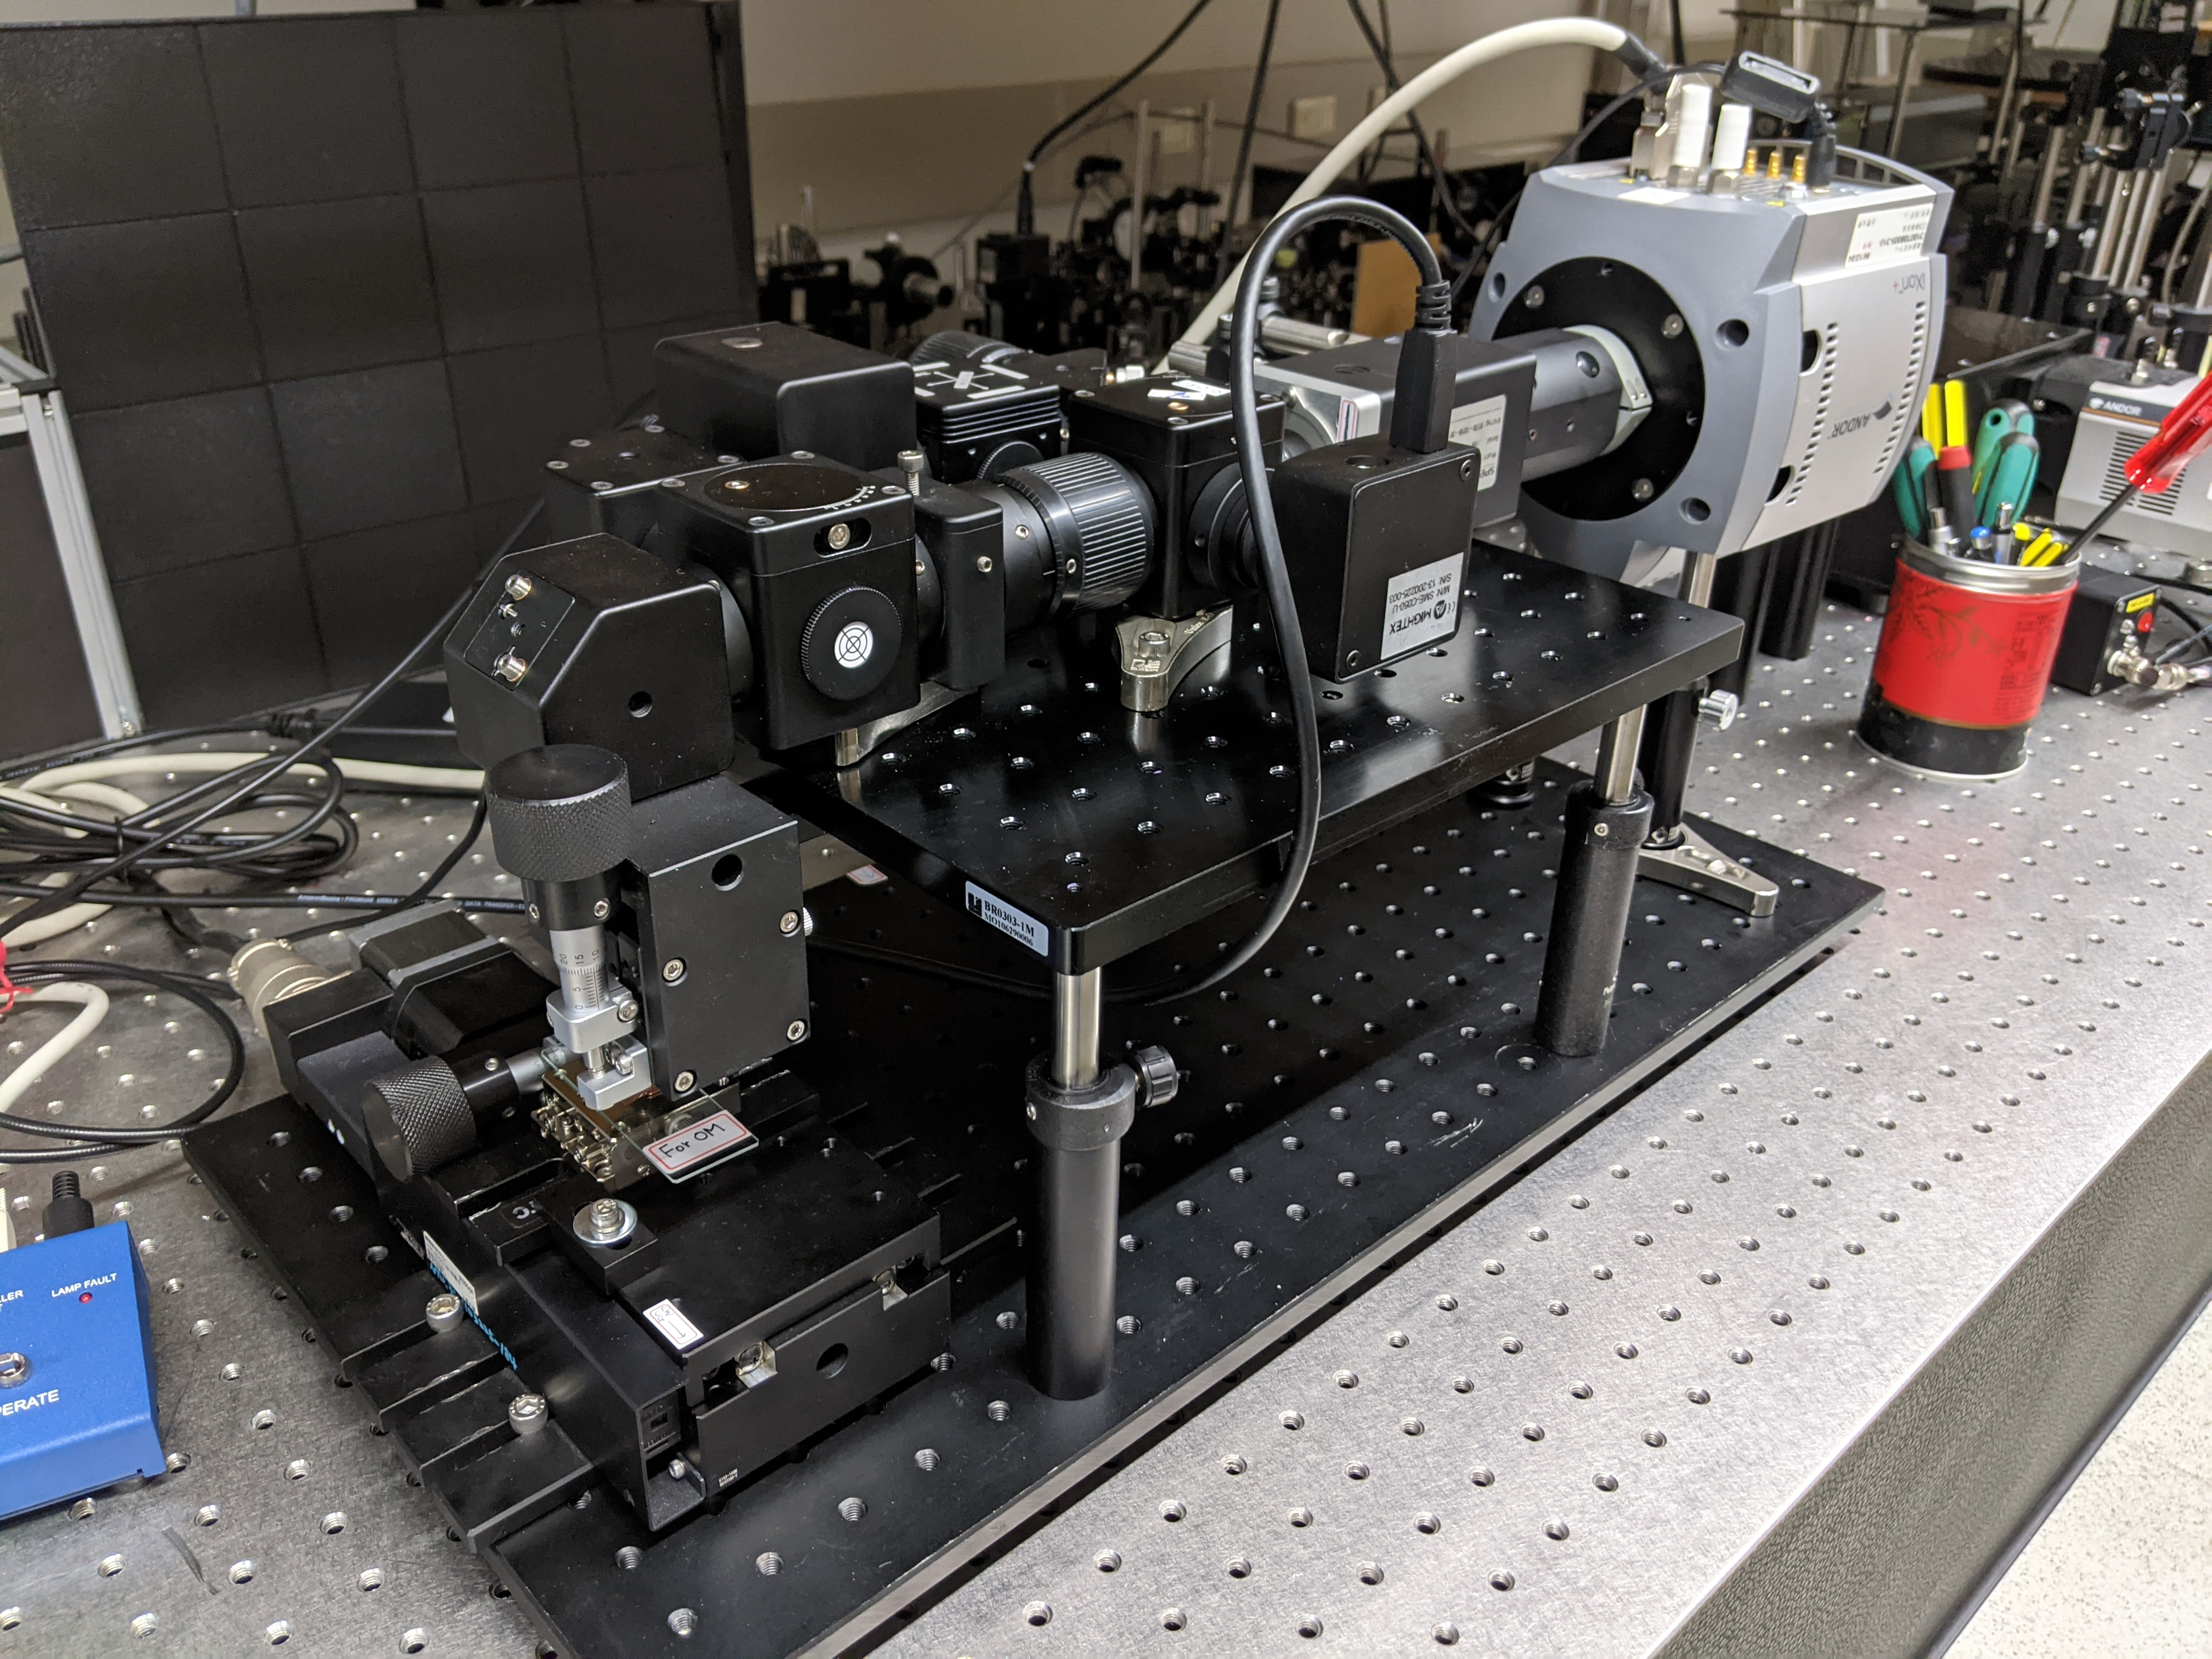
\includegraphics[width=\linewidth]{PXL_20210831_081957648.jpg}
        \caption{Micro system.}
    \end{figure}

    \subsection{Galvo}
    在最早的規劃中,第二階段的系統應該要從第一階段移動樣品的方式,改成以Galvo進行移動光源的方式掃描,但經過評估後,發現Galvo的運作方式並不適合線掃描系統。Galvo掃描的原理,是改變點光源照射在樣品上的位置,
    以一一對樣品上各個位置進行光譜量射。由於線掃描方式一次至少要將樣品上的整條掃描線完整照明,若以Galvo調動點光源的位置,則代表需要將光源在曝光時間內完整掃描一次樣品上的掃描線,並將掃描線上不同位置的像對應到狹縫上的不同位置。
    然後,這樣勢必代表仍必須以電動載台移動樣品,才能將樣品上不同位置的掃描線之影像成在固定位置的狹縫上,如此的作法與現階段以面光源照滿光學顯微鏡視野,並移動載台的方式,並無效率上的優勢,
    且以面光源照明尚有更方便使用者尋找ROI的優點。雖然以點光源方式理應可以相同的光源提供更強的照明,但在系統開發過程中亦沒有遇到照明強度不足的問題,因此就沿用第一階段以電動載台移動樣品的掃描方式。
    \subsection{照明}
    本系統現階段的照明設備,分別是高頻寬的Energetic LDLS與405 nm的DPSSL Laser,從兩個光纖collimator進入系統。照明光路的目標是希望能進樣擴大照明範圍,並使照明盡量均勻。
    然而在系統架設的初期,energetic的照明存在明顯的上下不均勻現象,如圖與圖的比較所示,圖是初期進行光陸校正時使用的HL-2000光源照明下的影像,可以看見將同樣的光纖接頭改接LDLS光源後,照明變得非常不均勻。
    且視野上下幾乎已經超出照明範圍。請這些都是在確認照明光路經過校正後的影像。
    \begin{figure}
        \centering
        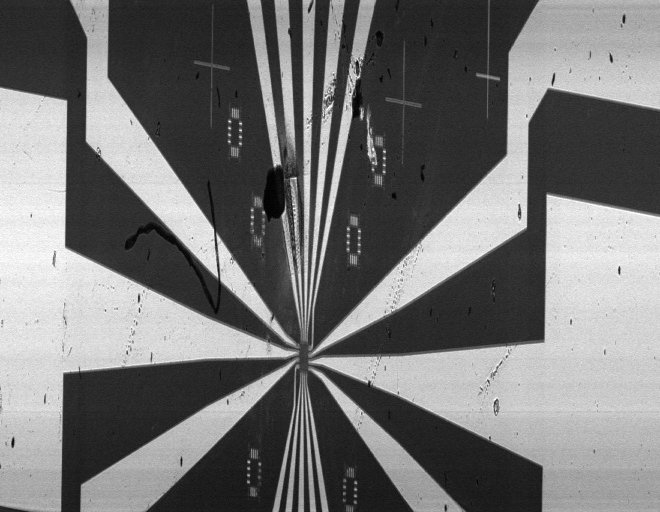
\includegraphics[width=0.5\linewidth]{0831focusForOmFullScanHL2000Scaled.jpg}
        \caption{HL-2000}
    \end{figure}
    \begin{figure}
        \centering
        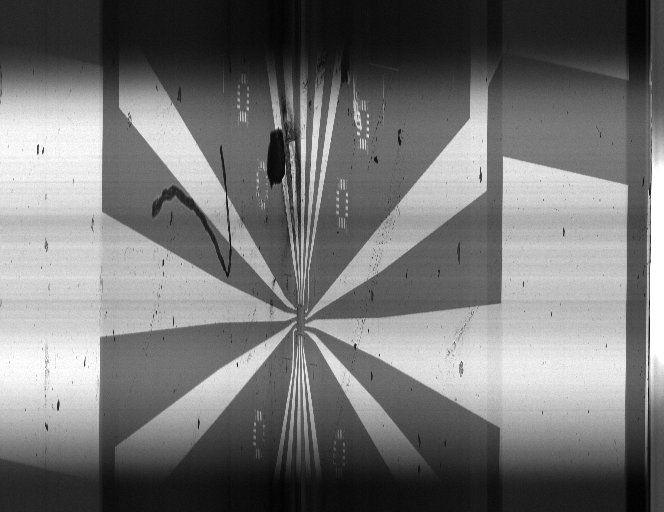
\includegraphics[width=0.5\linewidth]{0909Energetic.jpg}
        \caption{Energetic}
    \end{figure}
    為了改善照明的範圍,我們首先將原本使用的12.5cm tube lens換成現在所使用的15cm tube lens,希望能更集中使用成像中間較亮的部分,不過改善的效果有限,且系統上也沒有空間再裝設焦聚更長的透鏡。
    為了要進一步改善照明的均勻度,我決定嘗試調整LDLS光源系統內,光線進入光纖的Coupler,以及光線離開光纖,進入影像系統的Collimator。經過多次嘗試後,最終得出三種組態,可以藉此瞭解前述兩個組件對於照明的影響。
    \subsubsection{最高亮度、匯聚於背焦面} \label{section: illuOriginal}
    簡言之,平移調整光線進入光纖的Coupler,會決定LDLS的照明光譜中進入光纖的波段。該Coupler原先的狀態,是調整至照明亮度最高,也可視為是最寬的頻寬進入光纖的狀態。
    而光線離開光纖,進入照明系統的Collimator,即是一個可前後調整的透鏡,則會決定照明光源在影像系統內的何處匯聚。原先是調整至會剛好使照明光源正好匯聚在顯微物鏡背焦面的位置,使打在樣品上的光線為平行光。
    在這個設定下,掃描所得的影像如圖\ref{figure: brightest_on},可以看到影像上下明顯較暗,表示照明範圍還不夠大。從圖\ref{figure: om_brightest_on}的彩色OM影像可以看到,照明光源有類似色相差的情形出現,
    照明光源的影像不完整,且顏色也有分布偏移的情形。不過整體的照明尚算均勻,沒有明顯的干擾。
    \begin{figure}[t]
        \centering
        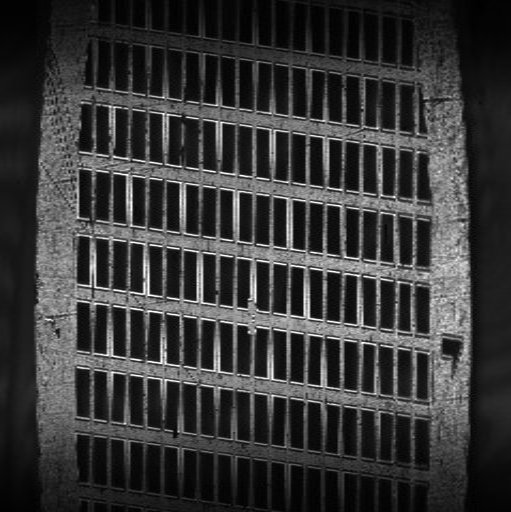
\includegraphics[width=0.5\linewidth]{on_brightest.jpg}
        \caption{Coupled at brightest, collimated on BFP.}
        \label{figure: brightest_on}
    \end{figure}
    \begin{figure}[t]
        \centering
        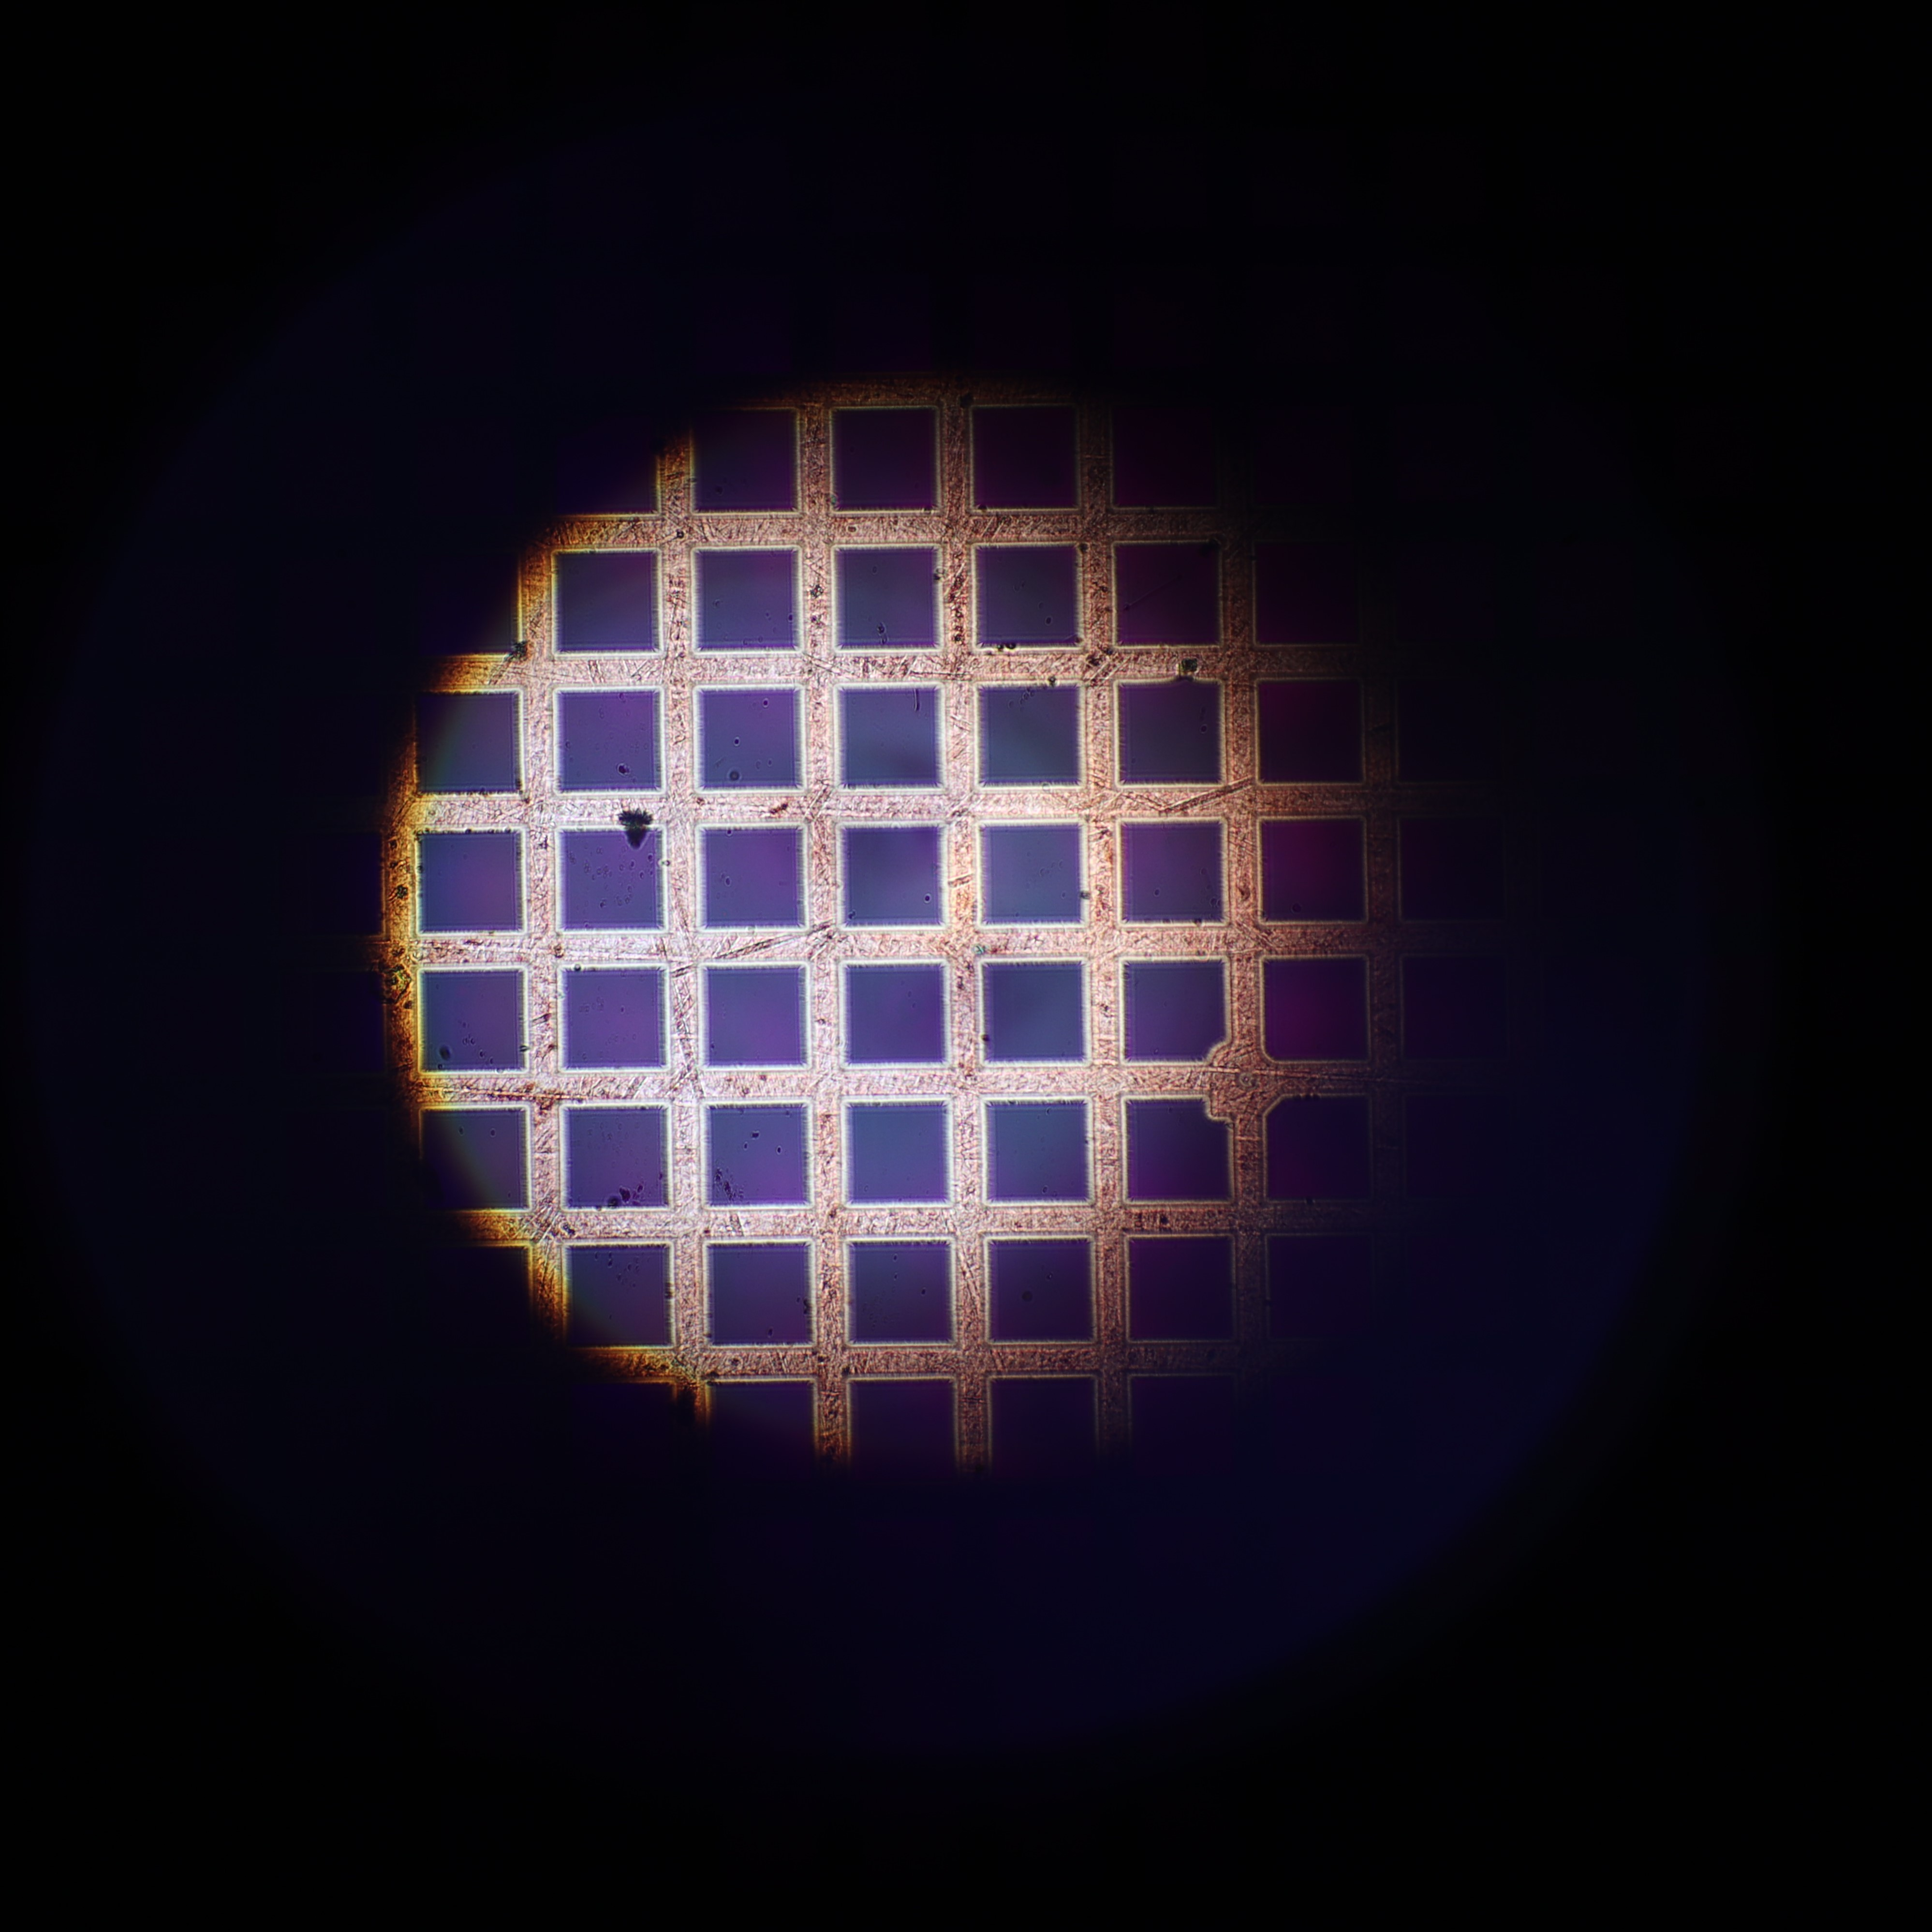
\includegraphics[width=0.5\linewidth]{om_on_brightest.JPG}
        \caption{OM: Coupled at brightest, collimated on BFP.}
        \label{figure: om_brightest_on}
    \end{figure}
    \subsubsection{最高亮度、不匯聚於背焦面}
    從前述的設定開始做調整,若將Collimator稍微調動,使光源不要匯聚在顯微物鏡的背焦面上,可以把照明的範圍再做擴大,並完整的照滿整個物鏡視野,如圖\ref{figure: brightest_off}、\ref{figure: om_brightest_off}所示,影像不再有上下明顯的暗帶。由於光線並未匯聚於物鏡的背焦面,打在樣品上的光線並非平行光,
    因此容易產生干擾的照明圖樣。以該螢光便樣品為例,由於螢光片半透明且具有厚度,不平行的光線穿過螢光片後,經反射後會產生不均勻的照明圖樣。
    \begin{figure}
        \centering
        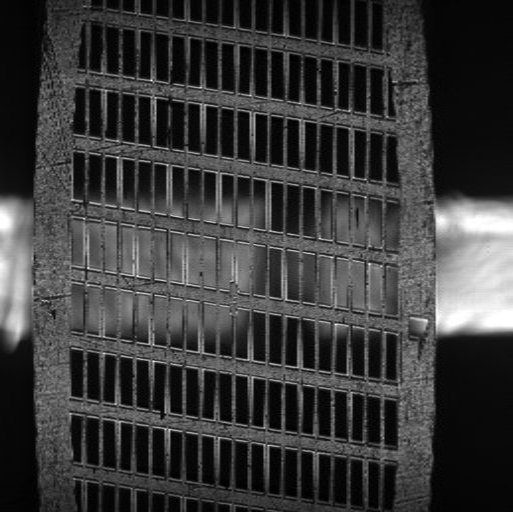
\includegraphics[width=0.5\linewidth]{off_brightest.jpg}
        \caption{Coupled at brighest, collimated off BFP.}
        \label{figure: brightest_off}
    \end{figure}
    \begin{figure}
        \centering
        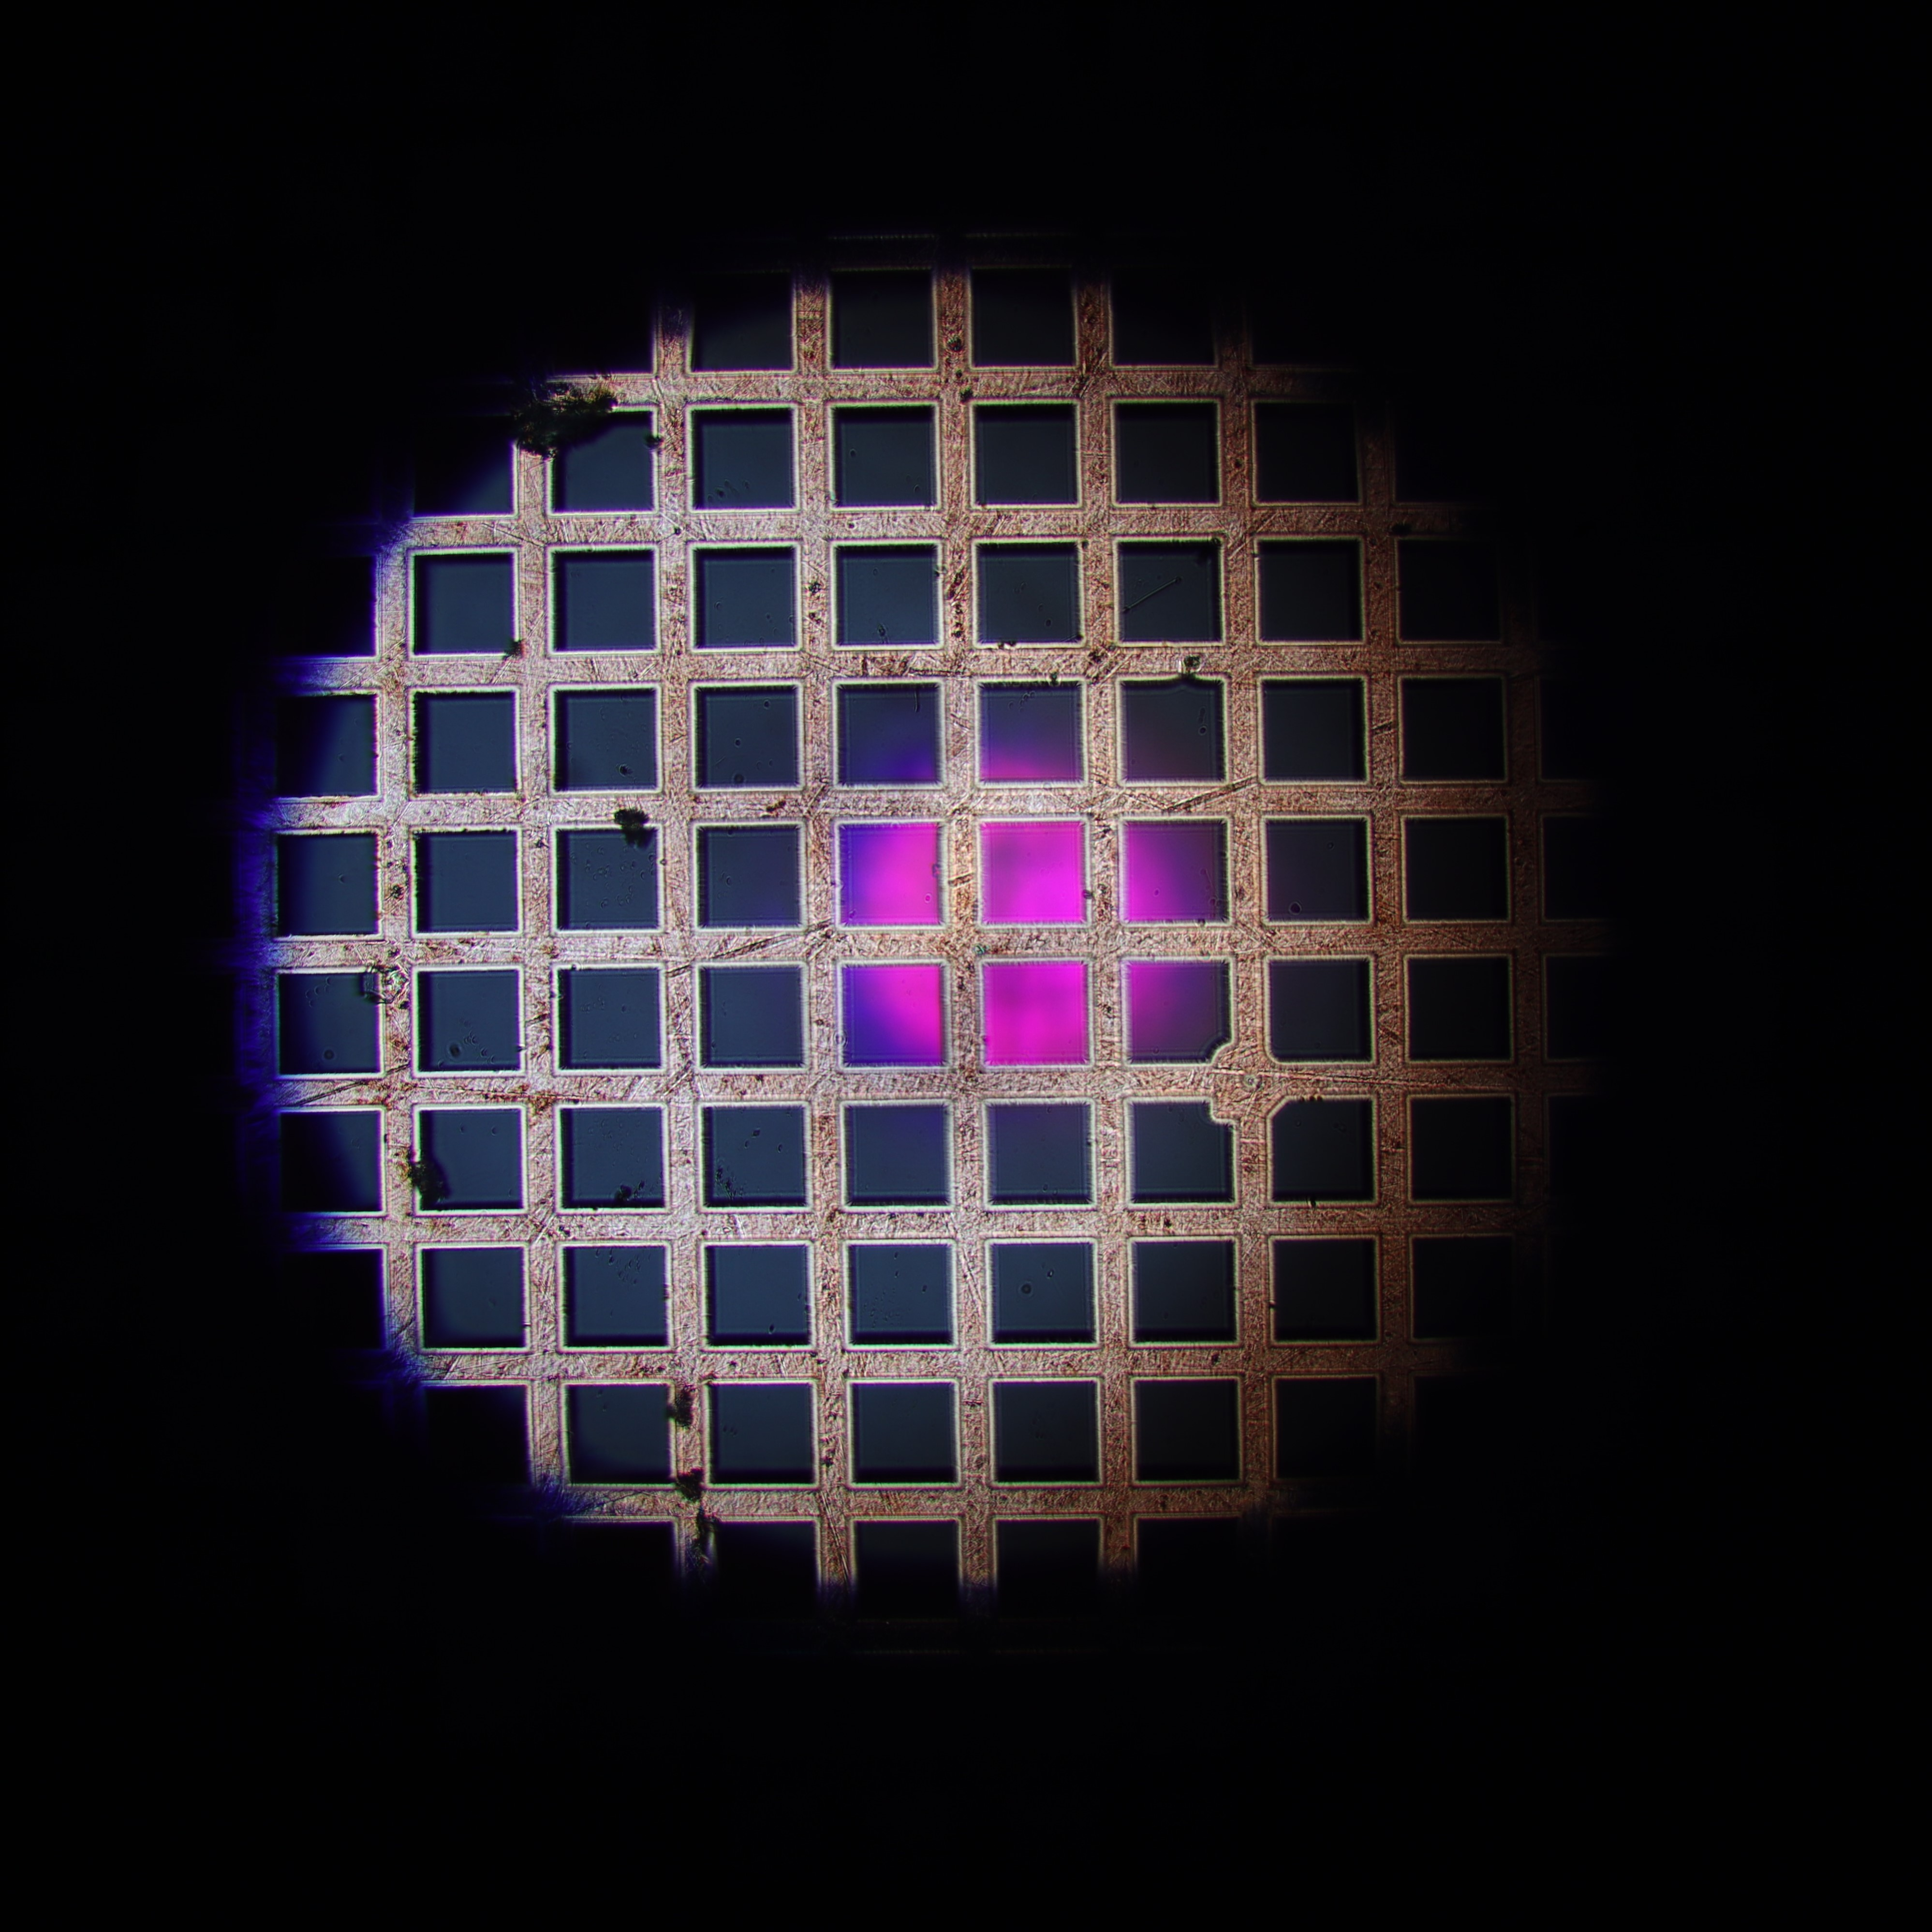
\includegraphics[width=0.5\linewidth]{om_off_brighest.JPG}
        \caption{OM: Coupled at brighest, collimated off BFP.}
        \label{figure: om_brightest_off}
    \end{figure}
    \subsubsection{較低亮度、匯聚於背焦面} \label{illuDark}
    為了避免上一個設定方式明顯的干擾紋路,我重新調整Coliimator,將光源匯聚至物鏡背焦面,並改為調整光纖的Coupler,以解決原初的設定中照明範圍不足的問題。在圖\ref{figure: evenest_on}、\ref{figure: om_evenest_on}中可以看見,
    經過調整後,照明關線的頻寬大幅減少,原先在\ref{section: illuOriginal}節中色相差的問題,幾乎完全消失,因此也確實可以完整的照明整個視野範圍,但由於實際進入光纖的光線已經減少許多,因此影像的整體亮度已有明顯的下滑。
    \begin{figure}
        \centering
        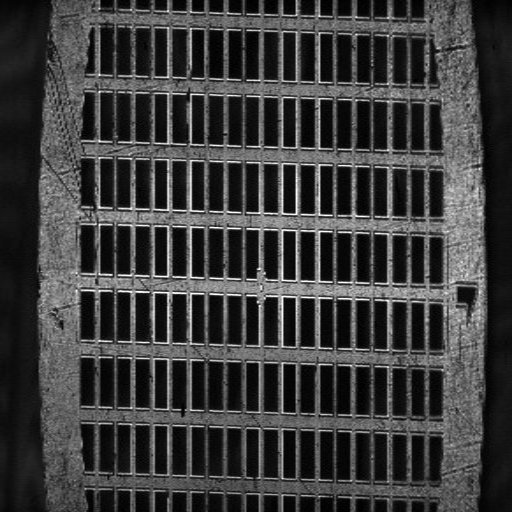
\includegraphics[width=0.5\linewidth]{on_evenest.jpg}
        \caption{Coupled at evenest, collimated off BFP.}
        \label{figure: evenest_on}
    \end{figure}
    \begin{figure}
        \centering
        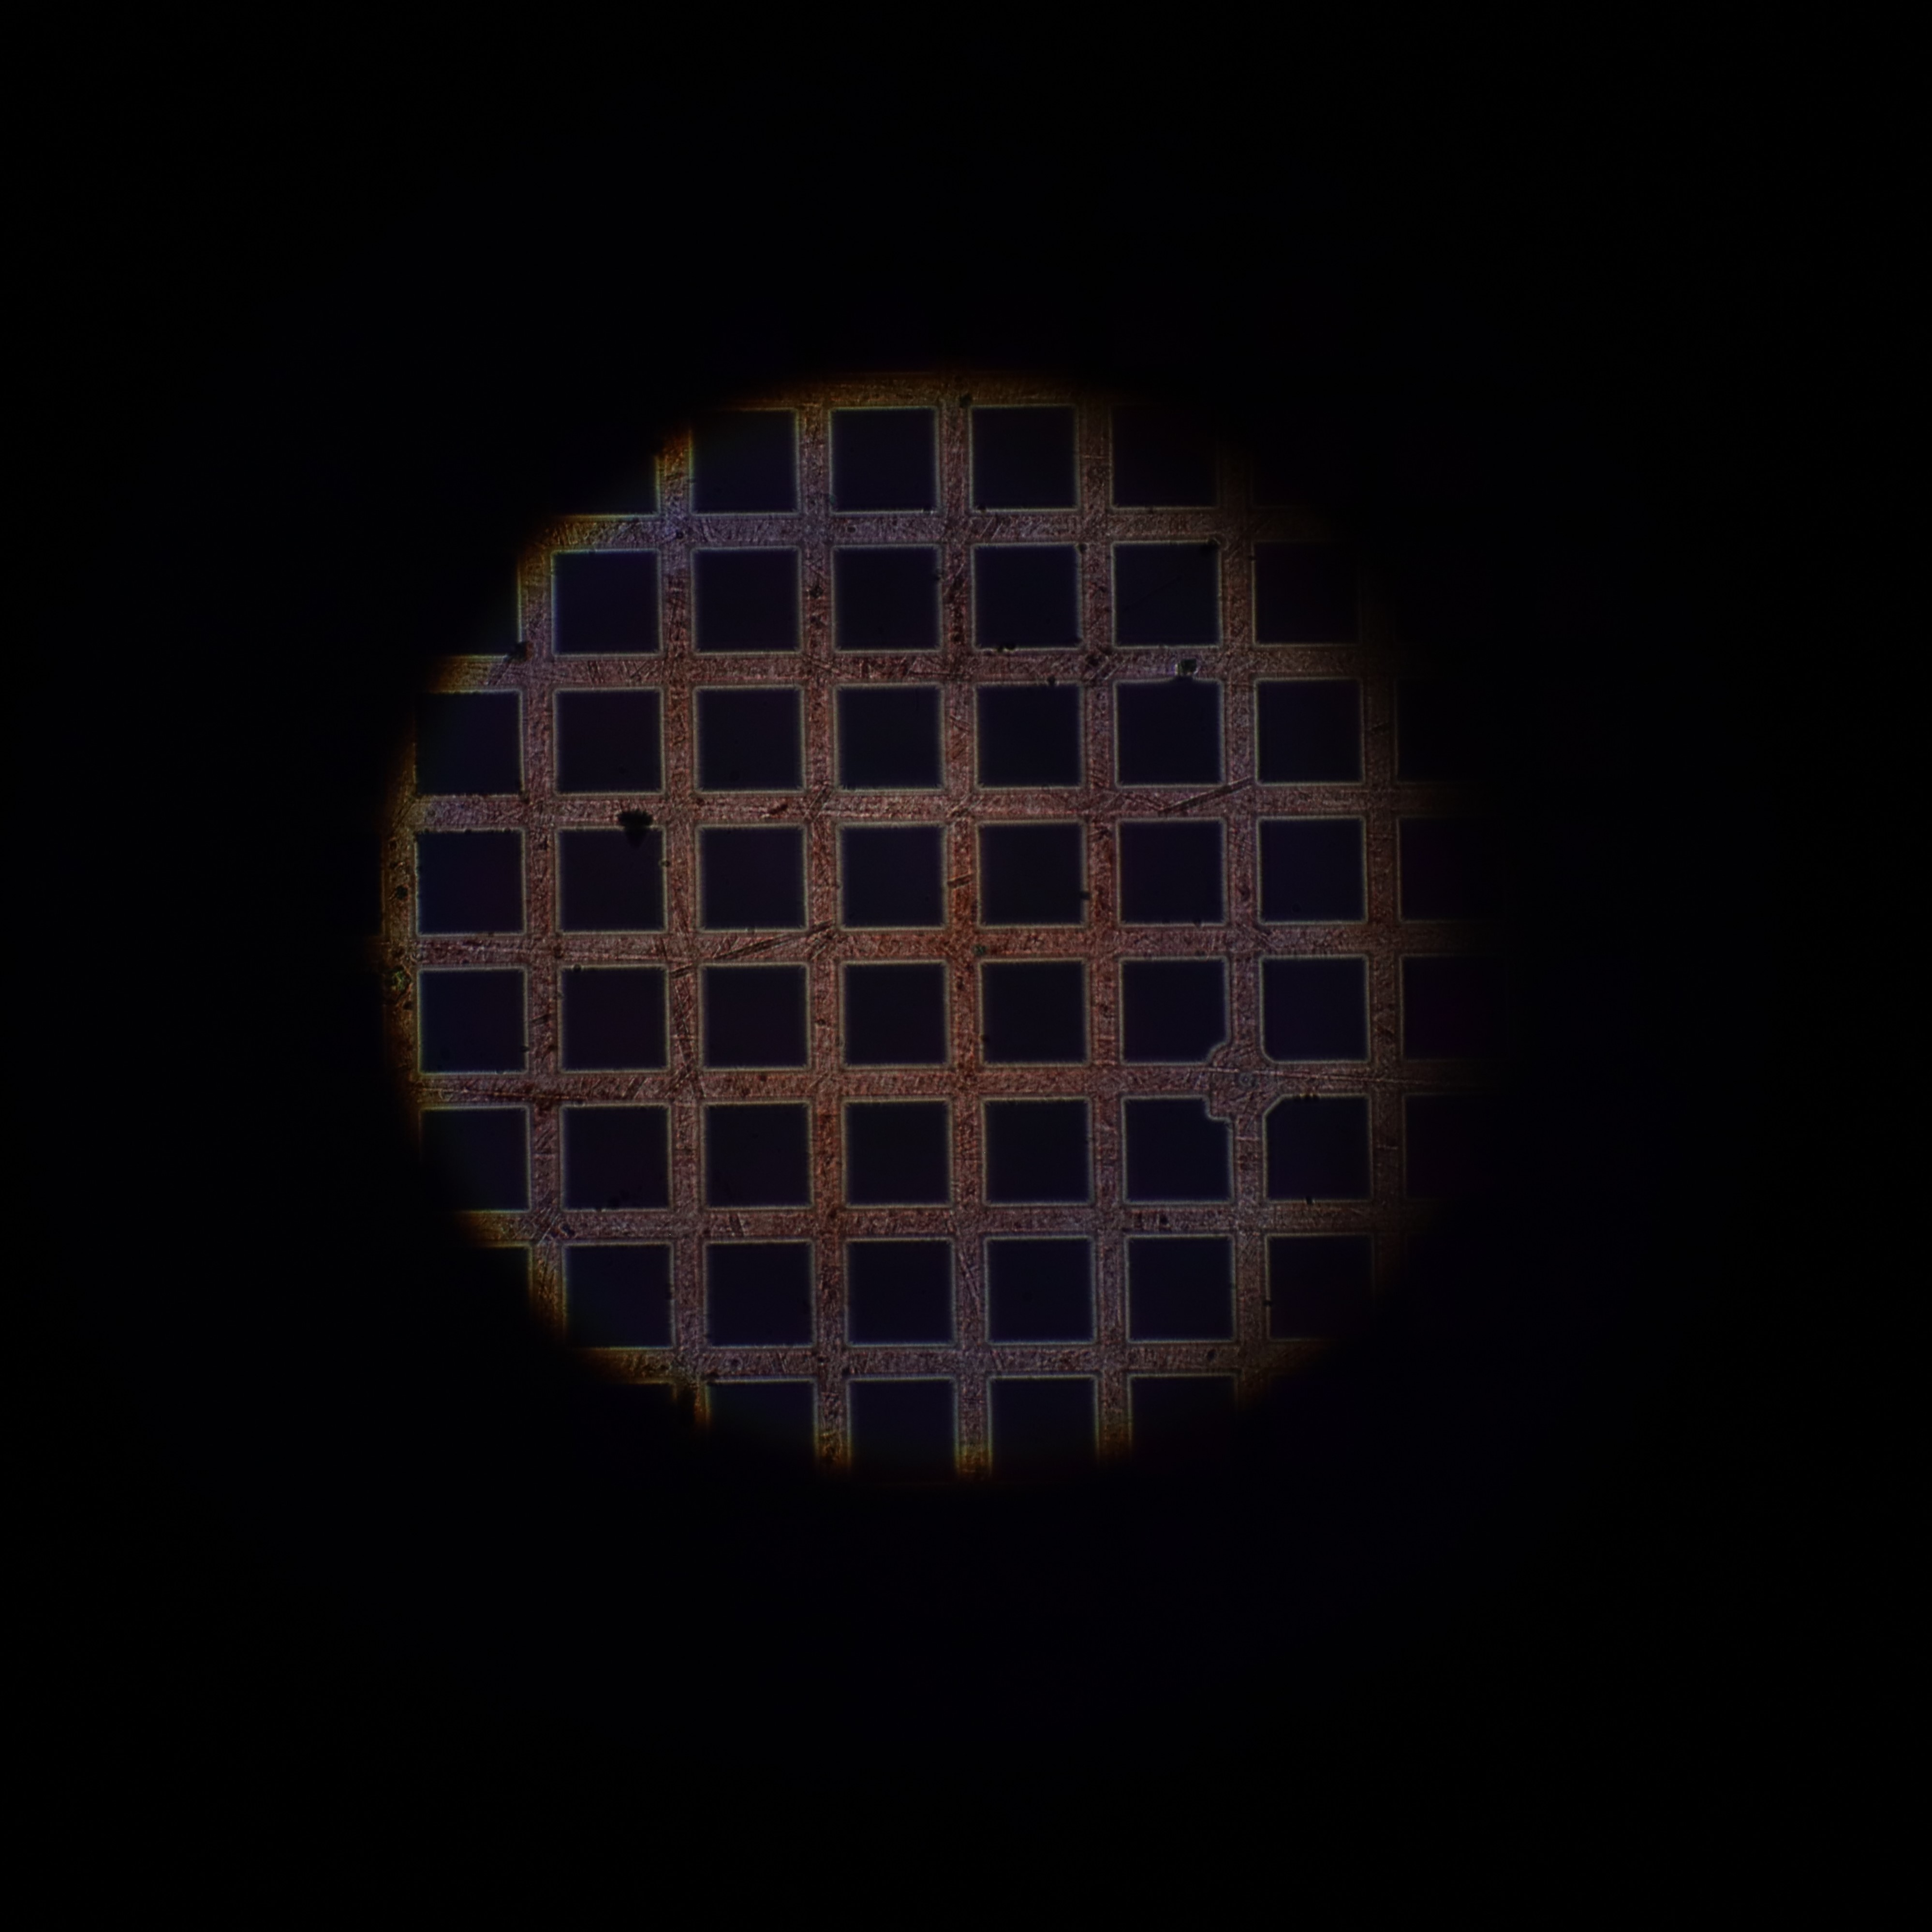
\includegraphics[width=0.5\linewidth]{om_on_evenest.JPG}
        \caption{OM: Coupled at evenest, collimated off BFP.}
        \label{figure: om_evenest_on}
    \end{figure}
    
    \noindent 綜上所述,照明的設定可以說是在光源光譜的完整度(頻寬)與照明範圍中做取捨,我們最後決定採取\ref{section: illuOriginal}節中的設定方式,
    雖然照明最後所得的影像會在上下有明顯的暗帶,但情形不算特別嚴重,且可以透過軟體進行後期處裡。若為了排除下上較暗的問題,而採取\ref{illuDark}的設定方式,形同於浪費了LDLS光源系統多數的光譜頻段,
    相形之下比上下的邊緣暗帶是更為嚴重問題,且也與我們因為需要更高頻寬的白光而使用LDLS的初衷背道而馳。
    \section{電動載台的操控}
    \subsection{初始校正}
    在開始進行開發前,首先以ORG1模式讓stage進行origin return\footnote{關於電動載台的origin return,請參閱controller的說明書。},經實測,從這個位置開始載台實際上並無法完整移動100000個pulse(在division number為1下,代表10cm),
    移動92550個pulse後就會觸碰到另一側的mechanical limit而停下。這應該是因為電動載台所偵測到的ORG訊號與CCWLS(ccw mechanical limit)訊號位置不同,實際上,ORG訊號會在CCWLS的CW側發生(也就是更早發生)。
    因此,從這個origin點開始,stage的移動範圍應該勢必會少於10cm。由於在顯微尺度下,應不會發生會使用到10cm掃描範圍的情況,故從這個origin開始,接著讓stage移動45000個pulse(4.5cm),將此點設為座標0,並把正負45000設為電動載台控制器的
    software limit,並寫入init檔中。經過測試,在這個範圍內電動載台都能正常移動。

    \subsection{原點復歸}
    init檔中Origin參數,紀錄的是目前的載台座標0點到mechanical limit的距離,這個mechanical limit是以ORG1 mode執行origin return後找到的mechanical limit。
    當使用者每次按下「set home」後,軟體會自動將目前所在的座標值與Origin參數相加,存為新的Origin參數,並計算在新的origin座標下,同樣位置的software limit的值,設定入controller中,並一併寫入init檔中。接著再把目前位置設為座標0點,完成set home程序。
    此時Origin參數紀錄的是新的座標0點,也就是目前所在位置,與mechanical limit的距離。而cwl與ccwl所記錄的,是在新的座標系統下,初始校正的software limit位置的新座標值,也就是說,
    經過set home之後software limit的位置永遠不變,只是座標值會隨著origin改變而改變。

    當使用者按下go home後,系統首先會以ORG1 mode執行origin return,接著移動到Origin參數所描述的距離,接著把該位置設為座標0點。如果你在操作過中,不小心關閉了stage controller的電源,會導致controller重設
    座標0點,此時只要執行go home,就能確保載台再次回到使用者透過set home所設定的座標0點。如果使用者一切的操作都正常,沒有在使用過程中關閉controller電源,都是在關閉軟體後才關閉電源,
    則載台的座標理應不會被重設,因為軟體的關閉流程中包括將載台移動到座標0點。使用者在操作過程中,如只是要將載台移動到座標0點,僅須透過普通的move left/right與可調的pulse數量即可輕易達成。
    \section{第二階段: 軟體}
    本階段的軟體開發主要集中在掃描功能的優化與完善。
    \subsection{使用者介面與功能}
    在軟體的前端介面上,我們希望讓使用者一目瞭然,能夠以最快的方式在螢幕上找到他所需要的控制項。因此將所有的控制按鈕分為數個類別,並從視覺上以背景圖塊(LabVIEW decorations)做出區別。
    另外,為了避免介面整體太過雜亂,在控制項的造型上都選用LabVIEW中內建與Windows系統風格一致的system控制項系列。因此整體的畫面簡潔,且不會有過多且不必要的視覺元素干擾使用者對整體介面的理解,
    僅輔以部分的silver decorations幫助使用者理解各類別控制項的分區,達到操作上直觀與美觀的目的。

    除此之外,操作介面除了靜態上的設計外,也有許多會需要因應使用者輸入來進行回應的動態變化。首先是希望使用者所有的輸入都能得到介面上的反應,讓使用者知道操作是否成功。另外,也盡量使用一些視覺元素,例如表達系統冷卻情形的顏色、載台移動中的燈號、矩陣旋轉的進度條等,
    來提醒使用者目前系統的狀態。這些動態的設計能避免讓使用者對於系統的操作狀態感到困惑。

    接著,雖然介面上布局排版不會在操作過程中有重大改變,但許多文字、圖表標題、尺規,會隨著顯示的內容不同,做出相應的變化。而在當下不應該被使用的控制項,也會在視覺上明顯的被淡化,
    從圖\ref{figure: acquire mode}與圖\ref{figure: scanning}的比較即可看到,進行掃描時所有的影像設定皆不應被更動,因此在介面上相關的控制項皆被淡化關閉。
    \begin{figure}
        \centering
        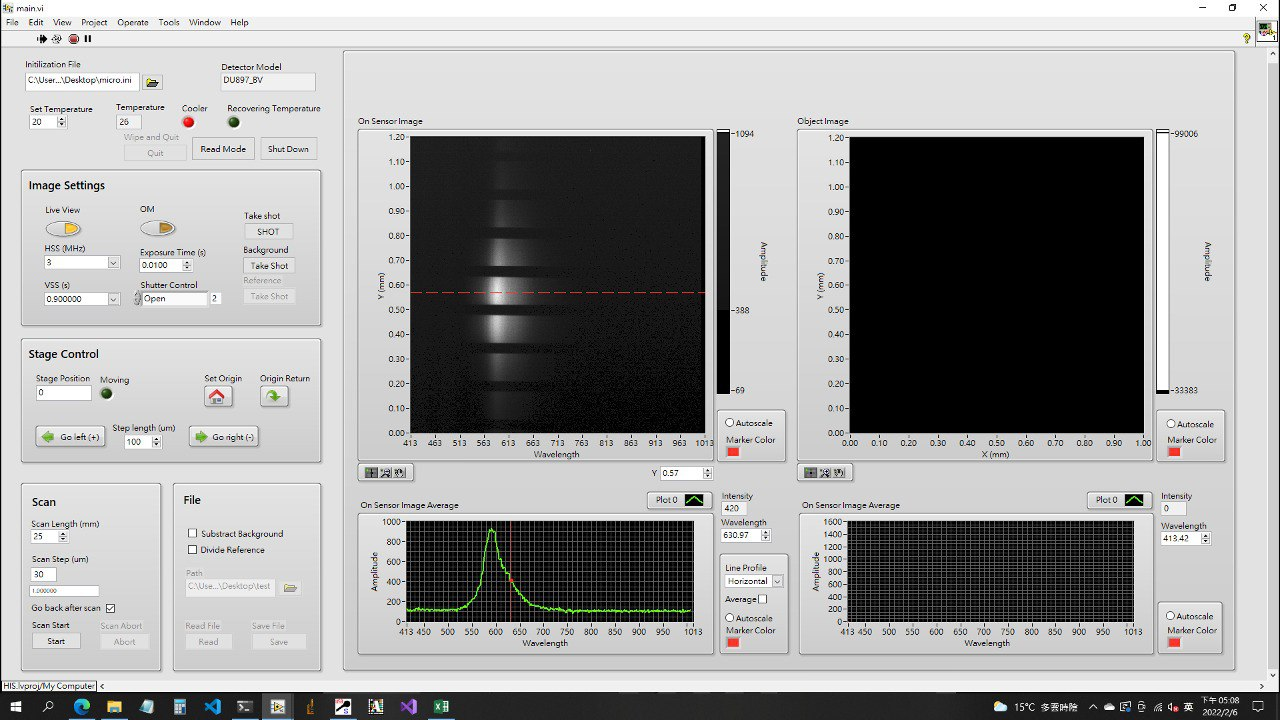
\includegraphics[width=\linewidth]{acquire.jpeg}
        \caption{在影像模式下的軟體介面。}
        \label{figure: acquire mode}
    \end{figure}
    \begin{figure}
        \centering
        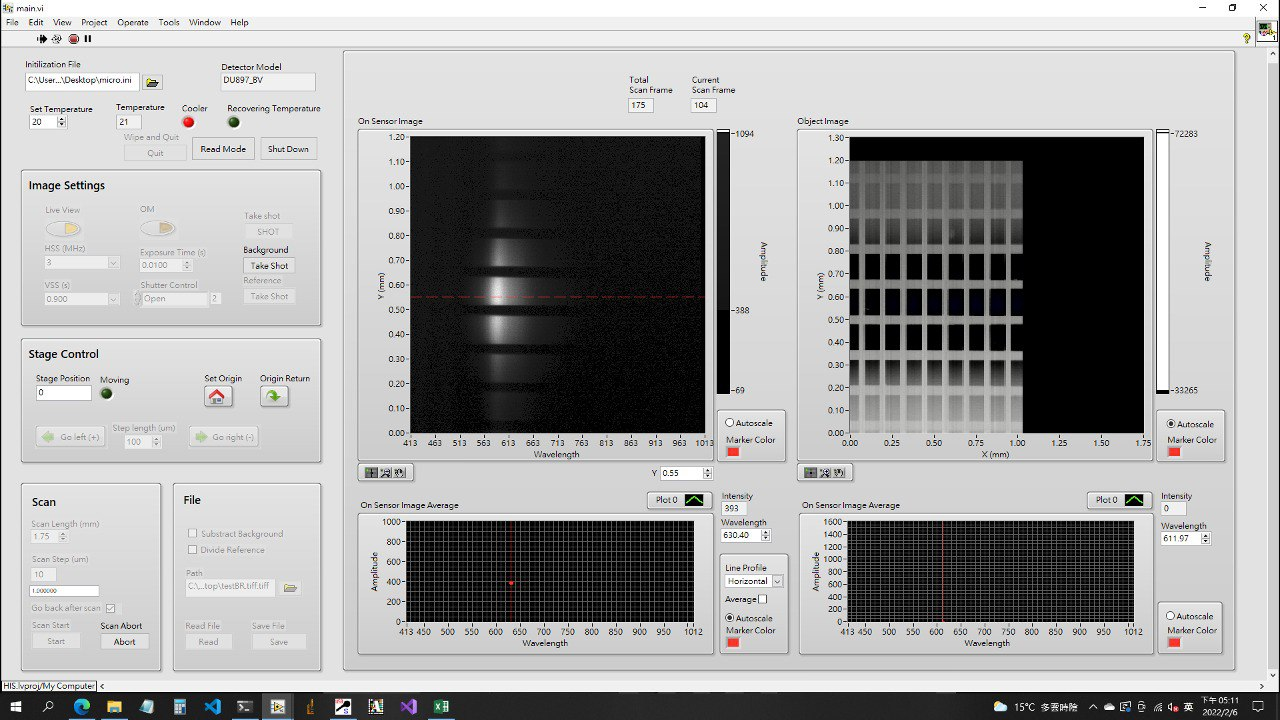
\includegraphics[width=\linewidth]{scanning.jpeg}
        \caption{掃描時的軟體介面。}
        \label{figure: scanning}
    \end{figure}
    \subsubsection{ROI框取}
    本階段中重要的軟體功能之一,就是圖\ref{figure: roi}中的ROI框取功能。當使用者打開OM影像畫面後,可以透過下方的拉桿調整掃描起始與結束的位置,接著只要按下ROI Scan,系統自動完成範圍內的掃瞄。
    該功能的開發過程中,最重要的是OM影像上所框取出的範圍,要如何轉換為實際的長度。我採用了一個已知大小的網格樣品,在我所設計的校正介面(Control\textunderscore demo.vi)中,讀取每個網格在螢幕上所佔的範圍大小,
    並以此來計算出螢幕與實際尺度的換算比率,並將這個比率儲存在.init檔中,請參考.init檔說明文件中的Scale Factor參數說明。

    除此之外,這個功能的開發,也牽扯到許多OM顯示的設計。由於我們並沒有使用到Canon M200影像感測器的全幅畫面,因此OM影像需先經過裁切,這些裁切的設定也都儲存在.init檔中,可以參考.init檔的OM章節。
    同時還要在OM影像上顯示線分光儀當下所觀測的位置(圖\ref{figure: roi}中白色垂直虛線),以及線分光儀的Y軸視野範圍(圖\ref{figure: roi}中兩條白色水明虛線),這些都需要以校正介面與具有已知特徵的樣品來協助判斷,
    在.init檔的說明文件中有較詳細的校正方法敘述。
    \begin{figure}
        \centering
        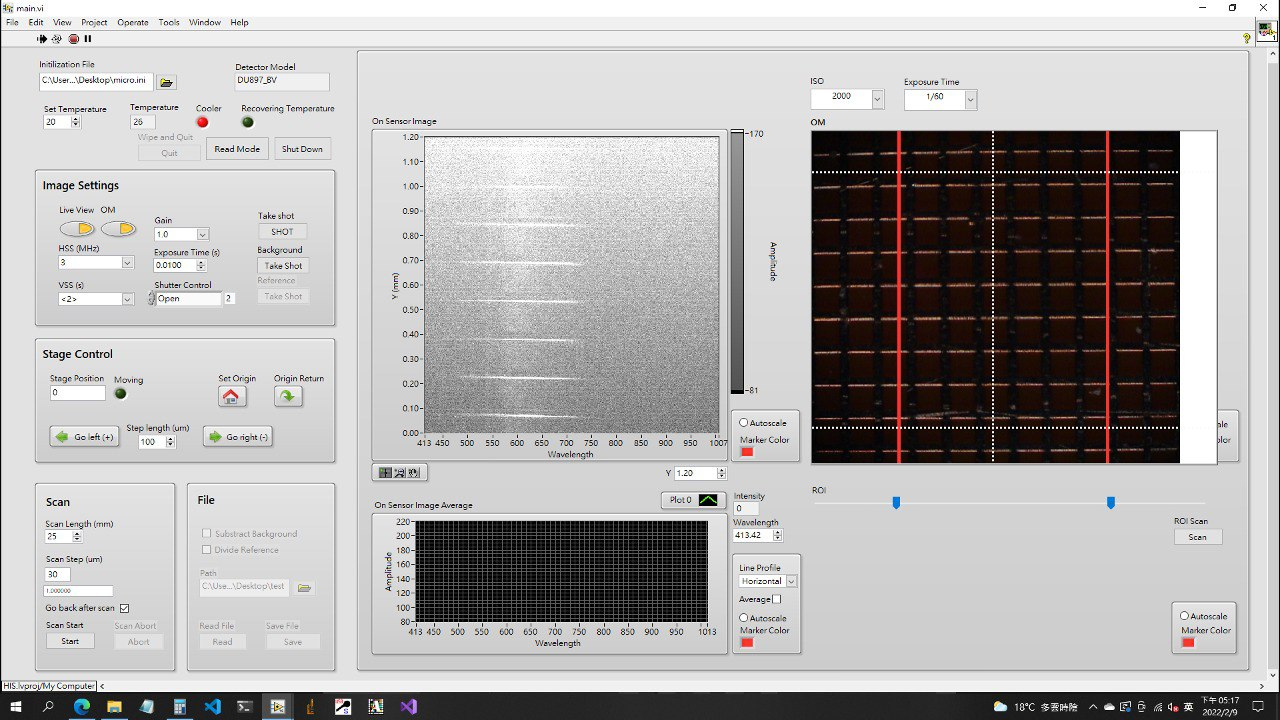
\includegraphics[width=\linewidth]{roi.jpeg}
        \caption{ROI框取功能。}
        \label{figure: roi}
    \end{figure}

    \subsubsection{背景/參考光譜}
    由於本系統以平行光進行照射的特性,非常適合作反射光譜的量測。然而,量測反射光表示我們必須對光源在光譜或空間中的不均勻進行校正,換句話說,我們希望量測的是樣品在各波長下的反射率,而非光譜本身。同時,在多數的光譜量測中,我們也都必須對量測系統的背景雜訊進行校正,
    因而著手開發背景光譜(背景雜訊)與光源參考光譜的擷取與校正功能。實際進行校正時,是將背景光譜(雜訊)油源資料中減去,再除以參考光譜。在操作的介面上,由於背景光譜幾乎可以適用於所有類型的光譜量測,而參考光譜只需要用於反射光譜的量測,因此我將其設計為兩個按鈕,可以分別進行擷取。然而需要注意的是,根據反射率的計算式
    \begin{equation}\label{equation: reflection}
        reflection \quad rate=\frac{measurement-background}{reference-background}
    \end{equation}
    若沒有擷取背景光譜,則參考光譜本身是無法用於校準的,因為參考光譜也必須減去背景雜訊後才能用於校準。因此介面的設計上,在沒有擷取背景光譜前,擷取參考光譜的按鈕將會是淡化且關閉的。

    使用者按下背景光譜按鈕後,系統會關閉iXon的快門,以當前所設定的影像參數拍攝一張張片,並顯示於右側螢幕,再將快門恢復至原本的狀態。該影像會被儲存到名為background.vi的FGV中,同時imagesetting.vi中的global variable hasBkg?會被設定為true。
    相似的,當使用者按下參考光譜的按鈕後,系統會開啟iXon的快門並以當前所設定的影像參數拍攝一張張片,該影像會被減去背景光譜\footnote{相減後數值小於0的矩陣元素會一律被設為0。},接著儲存到名為reference.vi的FGV中,同時imagesetting.vi中的global variable hasRef?會被設定為true。
    請特別注意,系統並不會強制使用相同的影像參數拍攝背景/參考光譜與掃描,這使使用者在某些特殊情況下可以自行決定拍攝背景或參考光譜的數值(例如拍攝參考光譜時反射面並不理想,可以用影像參數稍微彌補),但一般情形來說請務必確保這些影像以相同的參數拍攝。

    拍攝參考光譜時,使用者必須暫時將樣品改為一個反射面,確認對焦後,再拍攝參考光譜,以忠實擷取光源的樣貌。其餘對於掃描相關的操作皆相同,掃描完成後,將影像資料存進FGV(dataCube.vi)中時若hasBkg?與hasRef兩個全域變數有至少其一為true,
    系統就會在FGV內進行相應的校準運算,首先從background.vi中讀取出背景光譜,將掃描資料減去背景光譜,相減後所有小於0的矩陣元素會一律被設為0\footnote{我曾經試過相減後,將所有數值同步向上平移調整至矩陣中最小值為0,但這會導致相減的效果近乎消失。},
    接著再從reference.vi中讀取參考光譜,並將減去背景雜訊的掃瞄資料除以參考光譜\footnote{請注意reference.vi中的參考光譜為已經減去背景雜訊的參考光譜。}。

    掃描結束,FGV dataCube.vi的寫入完成後,進行影像瀏覽時,若hasBkg?與hasRef?兩個全域變數有至少其一為true,Data操作區就會出現substract background或與divide reference(若hasRef?為true)兩個checkbox,使用者勾選後,系統就會從FGV中讀取相應的影像資料。
    勾選substract backgroundc後,螢幕上所出現的影像與光譜皆會是減去背景雜訊後的光譜;相應的,勾取divide reference後,系統會自動將substract background也勾取,並且螢幕上皆會呈現反射率資料(式\ref{equation: reflection})。
    請特別注意,當使用者沒有勾選substract background時,是無法勾選divide reference的;同時,若使用者只有拍攝背景光譜(則hasRef?應為false),則也會無法勾選divide reference。
    \begin{figure}[ht]
        \centering
        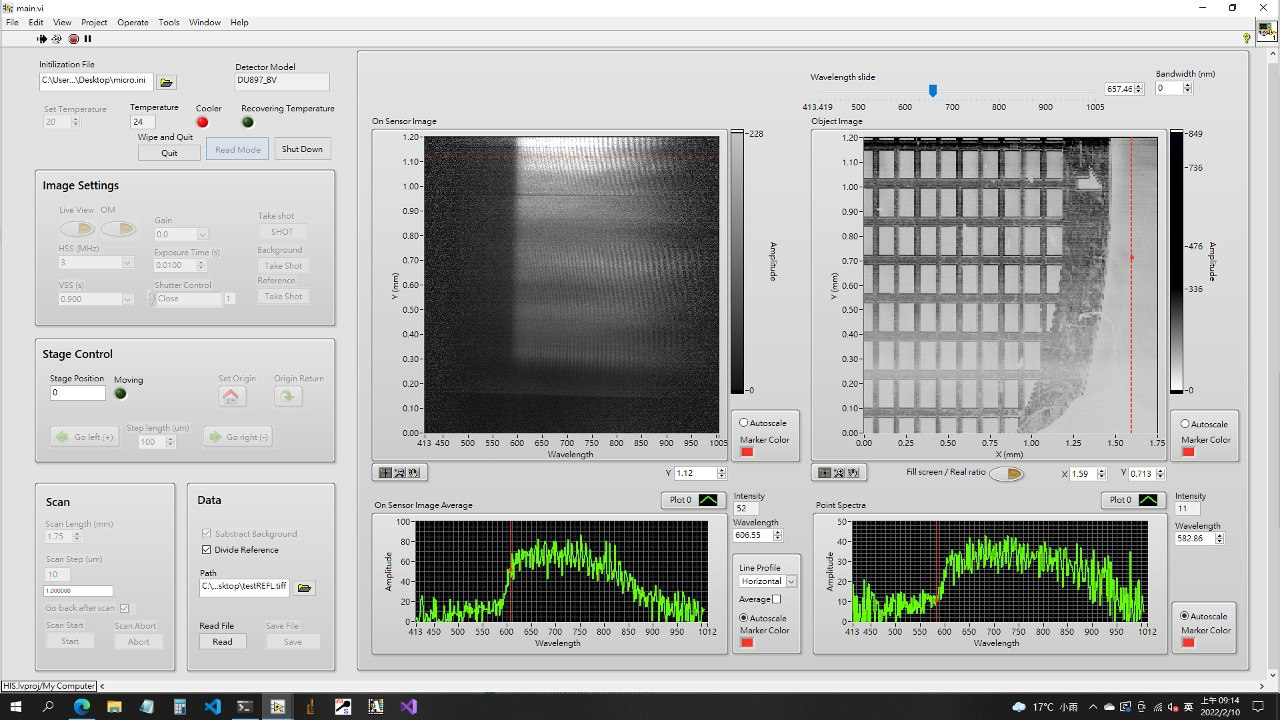
\includegraphics[width=\linewidth]{reflection.jpeg}
        \caption{檢視反射率影像時的軟體介面。}
        \label{figure: reflection}
    \end{figure}
    \subsection{.init檔}
    軟體的.init檔案,目標是將一些重要的參數,如系統的影像大小、xyz三軸的校正等,儲存在一個可以更改的文字檔案中,當系統的硬體有更動時,只要調整該.init檔案內的參數值,軟體就可以做出相應的改變,
    例如依據不同的影像尺寸進行記憶體的控管等。換句話說,透過init檔案儲存系統參數,就可以讓同一套軟體適用於不同的硬體上,只要檔案內的參數經過相應的調整即可。

    本系統的init檔共分為五個區段,分別儲存系統視野、iXon、電動載台、光譜校正與OM相關的參數。軟體在啟動時會將這些參數一次讀取,並儲存到相應的run-time變數中,以方便隨時取用。
    我們使用的檔案語法是LabVIEW內建的Configuration file VIs所產生的語法,其易於閱讀的特性,讓使用者可以直接透過一般的文字編輯器進行修改。其中某些參數,也會在軟體操作過程中由軟體自行做合適的修正。

    關於.init檔案的詳細使用說明,與每個參數所代表的意義和用處,請參閱本系統的.init檔說明文件(.init file documentaion of HSI system)。
    \subsection{軟體結構調整}
    隨著程式的軟體功能漸趨完備,操作上越來越複雜,各個功能所需的程式碼也都會佔去龐大的空間,使的程式碼的原檔變得過於冗長,變得非常難以閱讀與debug。且許多會重複使用、或是功能相近的程式碼也浪費了不少空間。
    另外,許多資料或變數必須在程式的不同區塊間傳遞,常常需要拉很長的data wire,且每個需要取用資料的地方都必須拉一條線,也造成資料流變得混亂。為了改善這些問題,並使後續的軟體開發更加便捷,我們決定將程式進行大規模的改造,將程式碼全部模組化,
    主程式只要控制UI與執行流程,其餘功能皆以subVI方式呼叫執行。另外,也以各種local variable、global variable與functional global variable來儲存並傳遞資料,使程式的
    資料流變的清楚明確。
    
    首先,將程式完全模組化,所有大小功能都以subVI funcation call來取代後,主程式的檔案尺寸縮減至一半,整體的程式碼也變得更加整齊、一目瞭然。在前端使用者介面完全不變的情形下,這些sunVI之間的API需要經過不少設計與調整,
    才能確保基本的運作都能以正確的參數完成,且必要的資訊資訊可以呈現在使用者面介面上。我們也使用了許多control reference的傳送,來使subVI能夠直接控制主程式上的使用者介面,這樣的操作方式減少了許多不必要的資料流,在整個模組化的過程中相當重要。
    我們也同時順便確立了程式的執行流程,在原始碼更易讀的情形下,更容易看出程式目前的所在階段,對於UI要因應不同階段的控制,也很有幫助。

    接著,我們將程式的資料流大幅精進。主要透過以下三種方式來操作:
    \begin{enumerate}
        \item 若是主程式內的UI相關資訊,例如使用者的滑鼠點擊位置,就以local variable來儲存,以方便主程式內不同的event或不同階段的程式取用資料。
        \item 若是.init檔或是影像擷取設定相關的資料就以project global variable的方式儲存,如此一來每一個subVI都可以自行對同一個變數進行讀取,能夠簡化API的設計。
        \item 最主要的data cube,以一個functional global variable的方式儲存,主要的原因是三維影像資料的數據較多,若以傳統的全域變數方式儲存,每次讀取時資料都會被複製一次,造成記憶體的浪費。
        另外,FGV能夠在資料儲存時一並執行程式,除了可以對racing的狀況進行處裡外,也方便做一些基礎的資料處理。
    \end{enumerate}
    \section{掃描速度}
    \subsection{掃描迴圈}
    為了要了解決定掃描速度的各個因素,首先要先說明整個掃描的行程是如何進行的。所謂掃描,其實就是在樣品的數個不同位置上以相同的參數拍攝線掃描影像,
    在使用者設定好掃描範圍與掃描步進(也就是每條掃描線之間的距離),電腦軟體會執行以下的迴圈,控制iXon與電動載台進行掃描:\textbf{首先},將電動載台移動到欲拍攝線掃描影像的位置,
    在每個迴圈中,這個移動的距離是固定的,也就是掃描步進。\textbf{接著},在確認電動載台已經移動到正確位置後,下指令使iXon開始擷取影像,確認iXon已經完成影像擷取後,iXon會將資料傳回電腦,
    程式並會進入下一次迴圈,重複執行以上動作的次數,是由程式以使用者設定的掃描距離與掃描步進進行計算。\textbf{迴圈次數執行完成後},電腦會將每條掃描線上所取得的線掃描影像接合成三維矩陣,為了確保該三維矩陣的「正面」是如肉眼所見的樣品影像,該矩陣還須經過旋轉,
    此矩陣旋轉的過程也需要時間。

    以下對於掃描時間的討論,皆是以一掃描範圍長3.5mm,掃描步進$10\mu m$(也就是總共拍攝350張線掃描影像並接合),曝光時間10ms的高光譜影像掃描為例。為了瞭解其他各項影像參數(HSS, VSS)對於掃描速度的影響,
    我調整iXon的HSS, VSS進行拍攝,並量測不同組合下所有迴圈執行完成所需的時間、迴圈執行後矩陣建立與轉向所需的時間,並以LabVIEW的precision timer(High Resolution Relative Seconds.vi)量測影像擷取完成後傳輸到電腦所需的時間。
    在以下的測試中,整個掃描迴圈中有三個等待時間,分別是等待電動載台移動至定點的時間,另一是等待iXon影像擷取完成的時間,以及等待iXon將資料傳輸到電腦所需的時間。這三個等待時間的設定方式如下所述:
    \begin{enumerate}
        \item 等待電動載臺: 電腦將電動載台移動的指令傳輸給電動載台控制器後,會等待\begin{equation} \label{eq: stageWait}
            \text{掃描步進}\times 200 \div 750 \quad milliseconds
        \end{equation},再進行迴圈內的下一個動作。
        \item 等待iXon擷取影像資料: 電腦在下指令給iXon進行影像擷取後,以一個while loop每1.5倍的曝光時間就詢問一次iXon的狀況,直到iXon回報擷取已完成後,才會進入迴圈內的下一個動作。
        \item 等待iXon傳輸影像資料: 電腦會等到「讀取iXon影像資料」的程式全部執行完成後,才會繼續迴圈內的下一個動作。
    \end{enumerate}
    再以上的設定下,所進行的測試結果如表\ref{tab: measuring}所示,表中的Pull sum代表350次迴圈中\textbf{等待iXon傳輸影像資料}所需時間的和,
    $t_1$代表350次迴圈執行所需的總共時間,$t_2-t_1$則是代表掃描結束後矩陣接合與轉換所需的時間。該測試提供了以下資訊,首先,若HSS頻率設定為1/3,掃描所需時間幾乎也會正好三倍,
    相對的,VSS對掃描的速度影響較小。HSS與VSS對於iXon運作的影響,可以參考iXon說明書的附錄。\cite{ixonManual}
    接著,\textbf{等待iXon傳輸影像資料}所需的時間極短,每張照片約1-2 milliseconds。最後,矩陣接合與轉換的時間雖然只與電腦的效能有關係,但所需的時間可能會占總掃描時間的將近1/3。
    \begin{table}[]
        \centering
        \begin{tabular}{lll||llll}
        HSS & VSS & Expo & Pull sum & Scan $t_1$  & $t_2$      & $t_2-t_1$  \\ \hline \hline
        3   & 0.9 & 0.01 & 554       & 44.1    & 01:28   & 43.9  \\ \hline
        3   & 1.7 & 0.01 & 502       & 45.25   & 01:10.1 & 25.55 \\ \hline
        3   & 0.5 & 0.01 & 581       & 43.76   & 01:09.7 & 25.94 \\ \hline
        1   & 0.9 & 0.01 & 497       & 01:48.9 & 02:20   & 71.1  \\ \hline
        1   & 1.7 & 0.01 & 633       & 01:50.0 & 02:16.2 & 26.2  \\ \hline
        1   & 0.5 & 0.01 & 588       & 01:48.7 & 02:13.9 & 25.2  \\
        (MHz)&(s)     &(s)    & (ms)         & (mm:ss)       & (mm:ss)       & (s)   
        \end{tabular}
        \label{tab: measuring}
        \caption{影像設定對掃描時間的影響。}
    \end{table}
    \subsection{速度提升}
    為了要使掃描的速度進一步加快,我們決定從前述的三個等待時間開始進行優化。首先,在前述的測試中已經顯示出,第三項\textbf{等待iXon傳輸影像資料}所需的等待時間極短,並不是決定掃描速度的關鍵因素。
    因此以下將集中討論\textbf{等待電動載臺}、\textbf{等待iXon擷取影像資料}兩個等待時間的調整。
    \subsubsection{電動載臺等待時間}
    原先用來計算電動載台等待時間的算式\ref{eq: stageWait},在其他掃描時被發現可能會有等待不足就下指令給iXon進行拍攝的問題,因此改以一個while loop,在下指令給電動載台控制器後,不斷詢問電動載台目前的狀況,
    直到控制器回報電動載台已經停下後,程式才跳出while loop並繼續下一個動作。然而,這樣的等待方式會造成掃描速度在各項設定下大致都變成表\ref{tab: measuring}的三倍,雖然最為保險,但其速度較難令人接受。
    最後,我們將電動載台的Drive speed (F)、acceleration/deceleration speed (R)、Startup speed (L)皆設為400,並且就「相信」電動載臺應該以400 pulse per seconds的速度前進,
    也就是說,我們可以確認電動載台的移動速度是400 micron per seconds(在division number為1的情形下),並以計算電動載台移動所需的確切時間。實務上,我還加上了10ms的等待時間做為緩衝。
    這樣的設定方式目前皆沒有遇到任何問題,且掃描時間也回復到表\ref{tab: measuring}中的速度。
    \subsubsection{iXon擷取影像資料的等待時間}
    如前所述,這段等待時間是以while loop不斷詢問iXon的方式決定,經過LabVIEW的precision timer量測後,發現以這樣的方式操作,在350張影像的掃描中,以表\ref{tab: measuring}第一列的參數設定,
    平均每張影像需要0.13213 seconds的時間iXon才會回報擷取完成。為了要減少這段等待時間,我們翻閱Andor SDK的說明書,希望能找到更快確認iXon影像擷取完成的方法,最後嘗試了下列幾項,羅列於此:
    \begin{enumerate}
        \item 使用Wait Acqusition 程式來取代while loop不斷詢問的方式,能將等待時間減少至0.119 seconds。
        \item 將while loop 中每次詢問的間隔時間拉長,對於等待時間沒有影響。以60 ms為例,反而使等待時間變長為0.154 seconds。
        \item 使用Wait Acqusition 程式,並且下指令讓iXon只擷取影像感測器上我們會使用到的區域(參見圖\ref{figure: image size}),等待時間減少至0.10662 seconds。
        \item 我曾資思考過以kinetic mode方式驅動iXon連續擷取影像,並設定很低的cycle time,讓iXon將影像存入buffer後就直接準備進行下一次拍攝,而不必先把影像在從buffer中讀出傳輸給電腦。
        但在同樣的影像設定下,Andor SDK的GetAcquisitionTiming所傳回的最低可設定cycle time,高達0.117 seconds,換句話說,這與單張影像方式驅動的等待時間是相同的。
        \item Andor SDK中有提供Crop mode,理論上可以提升iXon 的readout speed,但我們的iXon與控制板並不支援。另外也有Fast kinetic mode,會以sensor的一部份區域來做為暫存器,藉此提升速度,
        但由於我們須用到iXon sensor的整個高度,因此不適用。
    \end{enumerate}
    最後我們決定以3.的方式執行,影像感測器上所會用到的子區域則是定義於init檔中。
    \subsubsection{矩陣接合與旋轉}
    原先可能需耗費40秒進行的矩陣運算時間,在改以LabVIEW 的loop parrallelism操作後,能夠減少至約7秒的時間就完成。\footnote{不過該耗時仍與電腦的效能高度相關,實測在一樣的設定下,有可能僅需3秒即完成。}
    在經過以上的各式調整後,同樣進行350張線掃描,掃瞄範圍3.5mm,以0.01秒的曝光時間、0.9 HSS、3MHz VSS,掃描時間$t_1$正好為一分鐘,另約需4秒進行矩陣轉換,總計1:05即可完成掃描,並開始進行觀測。

    \section{第三階段: 軟體}
    本階段的軟體開發主要集中在影像資料的分析功能。
    \subsection{影像檔案讀取與進階存檔}
    \subsubsection{檔案讀取}
    本系統軟體截至目前為止皆以掃描功能為核心進行開發,只有在掃描結束後能對掃描的資料進行瀏覽,存檔並關閉後只能使用其他軟體來瀏覽掃描資料。為了讓使用者能有便捷的界面對過去掃描的資料進行瀏覽,我決定以
    原有的瀏覽介面,直接加上讀取檔案的功能。在開發上,讀取檔案的程式碼並不複雜。由節\ref{section: saveTiff}所述可知,Tiff檔案由影像資料標籤,與影像資訊本身組合而成。讀取Tiff檔案的方式相當直觀,
    首先讀取影像資料標籤,並透過影像資料標籤得知影像在檔案中的位置與大小,再讀取影像本身。不過由於我們所採用的為經過擴充之後的Tiff檔案,除了有公版的Tiff標籤外,尚有其他實驗室自行開發的軟體會需要的標籤,
    這些標籤分別儲存在兩個影像資料索引中(Image File Directory):公版IFD與實驗室的ULS IFD\footnote{IFD基本上就是將一群用途相似的影像資料標籤放在檔案中的相鄰位置,組成一個影像資料標籤的群組。},
    ,可以參閱lib/Halloween/Specification21\textunderscore01\textunderscore27HSI.xlsx檔案詳列本系統所使用到的影像資料標籤與影像資料索引。
    整體讀檔的操作順序大致如下所述。
    \begin{enumerate}
        \item 檔案起始處,跳過位元端序宣告\footnote{讀取檔案時理應先確認檔案寫入的端序設定,但由於本系統寫檔時一律以little-endian方式,因此讀檔時也一律採取little-endien設定,故不再讀取檔案起始處的端序宣告。}等數個位元組後(請參閱原始碼),即是公版IFD,從此處開始讀取基本的影像資料標籤。
        \item 因為每個影像資料標籤的大小皆為固定的12位元組,從此處開始每12個位元組即為一個影像資料標籤,依序讀取即可。
        \item 每個影像資料標籤皆依序包含:2個位元組儲存其ID(一個U16數字)、2個位元組儲存其檔案類型、4個位元組儲存其數量,剩下4個位元組儲存標籤資料本身。依此方式,即可讀出影像資料的ID,從前述.xlsx檔案即可對照出其意義,接著讀資料檔案型態後,即可以相應的方式將其最後幾個位元組的資料unflatten出來。
        \item 公版影像資料標籤中,有一個標籤是實驗室IFD的位置,從這個位置資訊即可以相同方式讀出所有必須的影像資料標籤。
        \item 公版影像資料標籤中,另有一個標籤是影像資料的位置(image strip offset),透過該位置資訊即可知道影像資料的位置,並存其他影像資料標籤計算出其大小,直接到該位置將正確大小的資料unflatten為正確大小的三維I32矩陣,所得的矩陣就跟剛掃描完時的矩陣擁有相同的性質,可以被原本的軟體直接讀取。
        \item 將該矩陣寫入dataCube.vi FGV中,就與剛掃描完時一樣,軟體即可以原本的方式讀取並呈現檔案中的資料。
    \end{enumerate}
    \subsubsection{建立「讀取模式」}
    有時使用者開啟軟體,僅是需要讀取檔案並瀏覽光譜,此時可以點按進入Readout Mode,系統即會跳過軟體的影像設定與掃描程序,直接進入瀏覽模式。此部分的程式與Shut Down按鍵相同,皆是透過控制while loop的離開來達成軟體程序的切換。
    另外,系統軟體開啟時,會自動啟動iXon的Andor SDK與Canon EDSDK,軟體會透過這兩個外部程式庫的執行錯誤來判定軟體系統是否有成功與硬體系統連接,並跳出視窗提醒使用者,同時也會避免對沒有連接的硬體系統下達指令,以避免更多錯誤產生。
    若軟體偵測到系統的主要影像感測器iXon沒有連接上,即會自動進入讀取模式。
    \begin{figure}[ht]
        \centering
        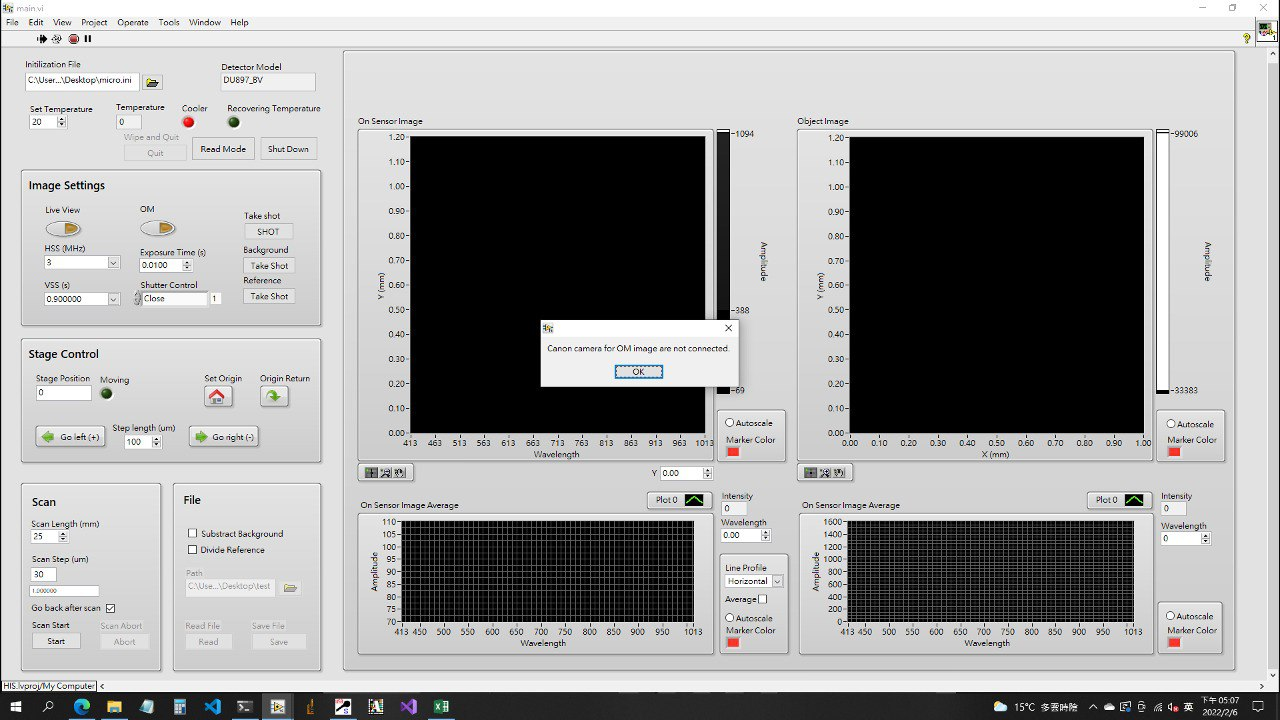
\includegraphics[width=\linewidth]{detectHW.jpeg}
        \caption{軟體會自行偵測硬體系統是否存在。}
        \label{figure: detect hardware}
    \end{figure}
    \subsubsection{TIFF格式之擴充}
    為了要使軟體在讀檔時能夠適當地調整UI,例如顯示實際掃描尺寸的圖標,並且在掃描影像檔案內儲存影像分析與比較時必要的資訊,我將原本的實驗室IFD內的影像資料標籤進行了擴充,可以參閱前述的.xlsx規格檔案,其中編號(ID)70-77者
    為本次所新增的標籤。要在存檔時新增標籤,可以如節\ref{section: saveTiff}所述一般以實驗室內原有的Tiff存檔程式庫進行操作即可。基本上,在SaveScan\textunderscore mk3.vi中,有一個ULSIFD subVI負責所有實驗室IFD影像資標籤的整理,
    只要在這個subVI內以newTag VI建立新的標籤,並以常數方式指定好標籤的ID、類型、數量、與內容即可。其中,標籤的資料內容需要建立起合適的API從主程式傳送到該VI內,我以一個cluster來將許多欲儲存的資料包裹起來傳送,
    並在這個VI中再進行unbundle,其中,project內的tiffHsiInfo.ctl與tiffInfo.ctl兩個type define即為了這個以cluster作為引數傳送的操作所建立。表\ref{tab: new tag}列出這次所新增的所有標籤,這些標籤都在實驗室IFD區段,讀取方式與原本的標籤亦都相同。
    \begin{table}[ht]
        \begin{tabular}{lllll}
        ID & Type    & No. & Content & Description \\
        70 & 4(U32)  & 1 & HSI: Step Length      & in um                   \\
        71 & 11(SGL) & 1 & HSI: Real Y Dimension & in mm                   \\
        72 & 11(SGL) & 1 & HSI: Real X Dimention & in mm                   \\
        73 & 11(SGL) & 1 & HSI: VSS of iXon      & in sec                  \\
        74 & 4(U32)  & 1 & HSI: HSS of iXon      & in MHz                  \\
        75 & 1(U8)   & 1 & HSI: bkg exist?       & 1 for true, 0 for false \\
        76 & 1(U8)   & 1 & HSI: ref exist?       & 1 for true, 0 for false \\
        77 & 11(SGL) & 1 & HSI: Gain             &                        
        \end{tabular}
        \caption{新增的影像資料標籤。}
        \label{tab: new tag}
        \end{table}
    \subsubsection{背景/參考光譜之儲存}
    參見SaveScan\textunderscore mk3.vi可以發現,若是掃描時backgroundExist或referenceExist為true,軟體會將背景光譜與參考光譜寫入在檔案的最後面。由iXon每次擷取影像時的影像尺寸皆為固定,
    因此背景/參考光譜影像的尺寸與其所需的位元組數量,也可以由其他影像資料標籤,如影像長寬與data cube層數等標籤得知,因此讀檔時軟體僅須由檔案最後,往回已推得的位元組開始讀取
    \footnote{此方式實非標準的tiff檔案寫入方式,只是較方便的解決之道。標準的作法應該是多建立新的tag,用以儲存背景/參考光譜影像的位置,讀檔時先從tag讀到影像的位置,再到該位置讀取影像。},
    即可讀出背景/參考光譜影像,並如掃描時一般,將其導入
    background.vi與reference.vi中。由於背景/參考光譜的校準是在dataCube.vi FGV中進行,且是該FGV偵測到backgroundExist或referenceExist為true時才會進行,因此將背景/參考光譜讀入相應的FGV之後,
    請確保backgroundExist或referenceExist已設為true,再將已經unflatten的三維掃描影像矩陣寫入dataCube.vi中,即可完成讀檔時的背景/參考光譜校準。
    \subsection{光譜瀏覽功能}
    在軟體介面中,共有兩個影像顯示螢幕與兩個光譜顯示螢幕,在這些顯示螢幕上,當畫面有顯示資料時,使用者可以與這些顯示螢幕以不同方式互動,來更仔細的瀏覽影像資料。最簡單的方式是以滑鼠點擊想要瀏覽的位置,
    軟體即會把該位置的光譜資料更詳盡的顯示出來。但軟體除了把該位置的光譜資料讀出外,也會在這些螢幕上顯示出一些相應的圖標,來輔助使用者了解目前正在進行瀏覽的資料,是從哪個位置所讀出。舉例來說,在瀏覽模式中,
    當使用者點擊右側螢幕上樣品影像的任一位置時,event structure中的right graph mouse down event中的程式,會在滑鼠點擊位置上畫上圖標,並換算且在畫面上顯示目前點擊的空間座標位置,來標示目前的瀏覽位置,並將滑鼠點擊位置轉換成目前顯示資料的array index,
    並以此index來讀取該位置的光譜,顯示在右側的光譜螢幕上,左側的影像螢幕則會顯示出該位置的線掃描光譜影像(on sensor image),若使用者點擊該線掃描光譜影像,程式會以event structure將滑鼠點擊位置送入drawIntensityGraph.vi中,
    此vi會將滑鼠點擊位置換算成array index,並畫上圖標,讀出該位置的line profile,並將其顯示在左側的光譜螢幕上。使用者在任何時候若點擊光譜螢幕,系統同樣會將滑鼠點擊位置送入另一個waveformGraphDraw.vi中,
    此vi會將滑鼠點擊位置換算成array index,並畫上圖標,讀出該波長下的強度,並把波長與強度顯示在畫面上。

    這些讀取滑鼠位置的vi與event structure內部的程式皆大同小異,首先會透過該螢幕的property node,讀出顯示幕在電腦螢幕上的所在位置與尺寸,並以此些資訊與得到的滑鼠點擊位置,
    換算出array index與空間座標(或是波長),將這些資訊回傳到主程式的control上,或是依index讀取相應的光譜。同時這些程式碼也會在正確的顯示螢幕上以一系列的draw picture functions畫出圖標。

    軟體畫面上負責顯示目前所點擊位置的空間與波長座標的這些control,也可以用來調整瀏覽位置。使用者可以直接輸入欲瀏覽的座標位置,或是以control上的increment/decrement小按鈕來做調整。
    當這些control的值被使用者以上述兩種方法更動時,軟體會以與前一段所述相同的方式呼叫相同的程式碼或vi,來重新繪製顯示幕上的圖標與各個顯示幕上所應顯示的資訊,需要特別注意的是,
    由於程式碼與vi皆是接收\textbf{滑鼠點擊位置}作為繪製與換算的參數,當使用者是直接更改這些座標值時,需先在event structure中把座標值換算成滑鼠點擊位置(跟前一段使用相同的property node),再送入這些vi或程式碼中。這麼做會因為多次換算時四捨五入的問題,
    導致換算出一樣的array index,因此需要一些case structure來做判定與換算的輔助。

    請特別注意,在這些相關的程式碼中,有一些while loop,是用來確保軟體不會顯示出不在波長軸校正陣列中的波長。iXon上波長軸的每一個pixel都代表一個波長,這是經過波長軸校正資料算出來的(見節\ref{section: z cali}),這些波長並會被儲存在一個陣列中,
    有時前述的程式碼會換算出不再這個陣列中的波長,程式會以這些while loop來尋找陣列中與換算值最接近的波長,將其顯示在螢幕上。

    \begin{figure}
        \centering
        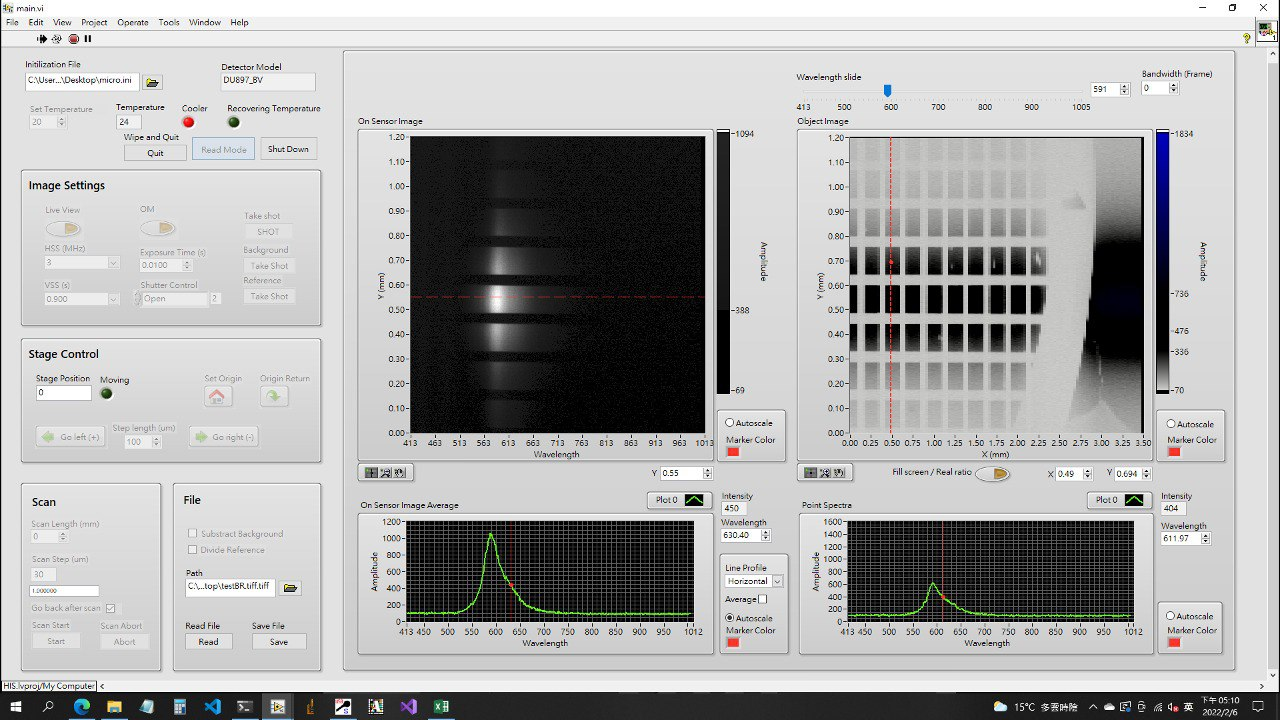
\includegraphics[width=\linewidth]{readmode.jpeg}
        \caption{軟體在讀取模式下的介面。}
        \label{figure: om_evenest_on}
    \end{figure}
    \section{已知問題}
    \begin{enumerate}
        \item \textbf{OM Camera Switch}: 本系統初期是使用Mightex小型相機作為OM影像的感測器,但由於其感測器尺寸比影像還小,限制了ROI功能的視野,因此後期換做Canon M200來做為OM相機,
        並以其來實作ROI功能。原初規劃要讓軟體能透過init檔在兩種相機中切換,但由於ROI功能所需的影像裁切功能參數,初期並未實現於Mightex相機的程式碼中。原本只是將兩套形式相同,但用於不同廠牌相機的程式已case structure切換,
        但由於ROI功能完成後基本上已不適用Mightex相機,因此原本的mightex程式碼就已Disabled diagram的方式續存於主程式中。若將這些diagram重新enable,理論上就可切換至mightex OM模式,但其對ROI功能的使用尚待調整。
    \end{enumerate}
\end{document}